%Dokumentinformationen
\newcommand{\titleinfo}{ProgCPP - Zusammenfassung, sowie weitere Autoren}
\newcommand{\authorinfo}{J. Brupbacher}
\newcommand{\versioninfo}{$Revision: $ \today}

% standard header
%Schriftgr�sse, Layout, Papierformat, Art des Dokumentes
\documentclass[10pt,twoside,a4paper,fleqn]{article}
%Einstellungen der Seitenr�nder
\usepackage[left=1cm,right=1cm,top=1cm,bottom=1cm,includeheadfoot]{geometry}
% Sprache, Zeichensatz, packages
\usepackage[latin1]{inputenc}
\usepackage[ngerman]{babel,varioref}
\usepackage{amssymb,amsmath,fancybox,graphicx,color,lastpage,wrapfig,fancyhdr,hyperref,verbatim}
\usepackage[T1]{fontenc}

\newcommand{\licence}{CC BY-NC-SA}

%pdf info
\hypersetup{pdfauthor={\authorinfo},pdftitle={\titleinfo},colorlinks=false}
%linkbordercolor=white
\author{\authorinfo}
\title{\titleinfo}

%Kopf- und Fusszeile
\pagestyle{fancy}
\fancyhf{}
%Linien oben und unten
\renewcommand{\headrulewidth}{0.5pt} 
\renewcommand{\footrulewidth}{0.5pt}

\fancyhead[L]{\titleinfo{ }\tiny{(\versioninfo)}}
%Kopfzeile rechts bzw. aussen
\fancyhead[R]{Seite \thepage { }von \pageref{LastPage}}

%Fusszeile
\fancyfoot[L]{\footnotesize{\authorinfo}}
\fancyfoot[R]{\footnotesize{\today}}
\fancyfoot[C]{\footnotesize{\licence \quad $\rightarrow$ \href{https://github.com/HSR-Stud}{Github: HSR-Stud}}}

%Programmausschnitte

\usepackage{listings}
%\usepackage{lstlinebgrd}

\definecolor{bgGray}{rgb}{0.95,0.95,0.95}
\definecolor{stringColor}{rgb}{0.16,0.00,1.00}
\definecolor{annotationColor}{rgb}{0.39,0.39,0.39}
\definecolor{keywordColor}{rgb}{0.50,0.00,0.33}
\definecolor{commentColor}{rgb}{0.25,0.50,0.37}

\lstdefinestyle{cpp}{ 
	%linebackgroundcolor={\ifodd\value{lstnumber}\color{bgGray}\else\color{white}\fi},   % choose the background color; you must add \usepackage{color} or \usepackage{xcolor}; should come as last argument
	backgroundcolor=\color{bgGray},
	basicstyle=\normalsize\ttfamily,        % the size of the fonts that are used for the code
	breakatwhitespace=false,         % sets if automatic breaks should only happen at whitespace
	breaklines=true,                 % sets automatic line breaking
	captionpos=none,                    % sets the caption-position to bottom
	commentstyle=\color{commentColor},    % comment style
	deletekeywords={...},            % if you want to delete keywords from the given language
	escapeinside={\%*}{*)},          % if you want to add LaTeX within your code
	extendedchars=true,              % lets you use non-ASCII characters; for 8-bits encodings only, does not work with UTF-8
	frame=tb,	                  	 % adds a frame around the code
	keepspaces=true,                 % keeps spaces in text, useful for keeping indentation of code (possibly needs columns=flexible)
	keywordstyle=\color{keywordColor}\bfseries,   % keyword style
	language=C++,                    % the language of the code
	morekeywords={*,...},            % if you want to add more keywords to the set
	numbers=none,                    % where to put the line-numbers; possible values are (none, left, right)
	numbersep=3pt,                   % how far the line-numbers are from the code
	numberstyle=\footnotesize\color{codeGray}, % the style that is used for the line-numbers
	rulecolor=\color{black},         % if not set, the frame-color may be changed on line-breaks within not-black text (e.g. comments (green here))
	showspaces=false,                % show spaces everywhere adding particular underscores; it overrides 'showstringspaces'
	showstringspaces=false,          % underline spaces within strings only
	showtabs=false,                  % show tabs within strings adding particular underscores
	stringstyle=\color{stringColor},     % string literal style
	tabsize=2,	                   % sets default tabsize to 2 spaces
	title=\lstname                   % show the filename of files included with \lstinputlisting; also try caption instead of title
} % ./header.tex nicht editieren (Projekt LaTeX-Header benutzen)

%%%%%%%%%%%%%%%%%%%%%%%%%%%%%%%%%%%%%%%%%%%%%%%%%%%%%%%%%%%%%%%%%%%%%%%%%%%%%%%%%%%%%%%%%%%%%%%%
% Neue Befehle und Definitionen                
%%%%%%%%%%%%%%%%%%%%%%%%%%%%%%%%%%%%%%%%%%%%%%%%%%%%%%%%%%%%%%%%%%%%%%%%%%%%%%%%%%%%%%%%%%%%%%%
% This is needed for one more subsection, ex. 1.1.1.1, is called by \paragraph{}
\usepackage{titlesec}
\setcounter{secnumdepth}{4}
\setcounter{tocdepth}{4}
\titleformat{\paragraph}
{\normalfont\normalsize\bfseries}{\theparagraph}{1em}{}
% Settings which are used to set the distance above and under the sections
%\titlespacing*{\paragraph}{0pt}{2.25ex plus 1ex minus .2ex}{1.0ex plus .2ex}
\titlespacing{\section}{0em}{0.5em}{0.5em}
\titlespacing{\subsection}{0em}{0.5em}{0.5em}
\titlespacing{\subsubsection}{0em}{0.5em}{0.5em}

% Linksbündig
\setlength\parindent{0ex}

% This is needed for a smaller itemlist, is called by \compactenum {}
\usepackage{paralist}

% This is needed for merging some columns in a table
\usepackage{multicol} 
\usepackage{multirow}

% This is needed for code listing
\usepackage{listings}

% This is needed for UML Diagrams
\usepackage{tikz}
\usepackage{pgf-umlcd}

% Courier font
\usepackage{courier}

\definecolor{red}{rgb}{1,0,0}
\definecolor{blue}{rgb}{0,0,1}
\definecolor{black}{rgb}{0,0,0}
\newcommand{\verweisc}[1]{$_{\textcolor{red}{\mbox{\small{C Kap. #1}}}}$}
\newcommand{\verweiscpp}[1]{$_{\textcolor{blue}{\mbox{\small{C++ Kap. #1}}}}$}
\newcommand{\verweisboth}[2]{$_{\textcolor{red}{\mbox{\small{C Kap. #1}}}}$$_{\textcolor{black}{\mbox{\small{, }}}}$$_{\textcolor{blue}{\mbox{\small{C++ Kap. #2}}}}$}
\newcommand{\verweishoch}[1]{${\textcolor{red}{\mbox{\small{Kapitel #1}}}}$}
\newcommand{\lc}[1]{\textit{\texttt{#1}}}

%Document Anfang
\begin{document}	

	\title{\fontsize{50}{60}\selectfont ProgCPP}
	\maketitle
	\thispagestyle{empty}	% no page number on title page
	\vspace*{0.5cm}
	\begin{center}
		\includegraphics*[width=0.7\textwidth]{pics/2000px-ISO_C++_Logo.png}
	\end{center}
	\vspace*{2cm}
	Auf Vorlage der Zusammenfassung von L. Leuenberger, M. Ehrler, C. Ham, L. Däscher aus FS14 und der Vorlesung von R. Bonderer aus FS19. Die ganze Zusammenfassung richtet sich nach der \lc{C++11} Version.
	\newpage
	\setcounter{tocdepth}{2}
	\tableofcontents
	\newpage
	\raggedbottom
	\lstset{style=cpp}

	\section{Ein- und Ausgabe}
	Um die \lc{C++} Ein- und Ausgaben nutzen zu k�nnen, muss man die Bibliothek iostream einbinden. Das geschieht mit:
	\lstinputlisting{code/iostream.cpp}
	Damit die Ein- und Ausgabebefehle auch wirklich genutzt werden k�nnen, m�ssen sie mithilfe von
	\lstinputlisting{code/using_namespace_std.cpp}
	noch bekanntgegeben werden.\newline	
	\begin{minipage}[t]{11 cm}		
		\subsection{Streamkonzept}
			\begin{compactitem}
				\item Ein \lc{Stream} repr�sentiert einen sequentiellen Datenstrom.
				\item \lc{C++} stellt 4 Standardstreams zur Verf�gung:
					\begin{compactitem}
						\item \lc{cin}: Standard-Eingabesteam
						\item \lc{cout}: Standard-Ausgabestream
						\item \lc{cerr}: Standard-Fehlerausgabestream
						\item \lc{clog}: mit \lc{cerr} gekoppelt
					\end{compactitem}
				\item Alle diese Streams k�nnen auch mit einer Datei verbunden werden.	
				\item Alle Schl�sselw�rter m�ssen immer ganz links auf der Zeile stehen!\newline
			\end{compactitem} 
	\end{minipage}
	\hspace*{0.5cm}	
	\begin{minipage}[t]{7 cm}
		\subsection{Eingabebeispiele}
			\lstinputlisting{code/eingabe_3.cpp}	
	\end{minipage}
	\hspace{0.5cm}
	\subsection{Ausgabebeispiele}
		\lstinputlisting{code/ausgabe_3.cpp}
		\lstinputlisting{code/ausgabe_4.cpp}
		
	\subsection{Formatierte Ein- und Ausgabe: Manipulatoren ohne Parameter}
	\lc{ios}, eine Basisklasse von \lc{iostream}, stellt verschiedene M�glichkeiten (Format Flags) zur Verf�gung, um die Ein- und Ausgabe zu beeinflussen.\newline
		\begin{minipage}[t]{7 cm}
			\subsubsection{boolalpha} 
				\lc{bool}-Werte werden textuell ausgegeben.
				\lstinputlisting{code/boolalpha.cpp}
		\end{minipage}
		\hspace*{0.1cm}	
		\begin{minipage}[t]{2 cm}
				\vspace*{1.2cm}\lstinputlisting{code/boolalpha_aus.cpp}
		\end{minipage}
		\hspace*{0.3cm}	
		\begin{minipage}[t]{7 cm}
			\subsubsection{showbase} 
				Zahlenbasis wird gezeigt.
				\lstinputlisting{code/showbase.cpp}
		\end{minipage}
		\hspace*{0.1cm}	
		\begin{minipage}[t]{2 cm}
				\vspace*{1.2cm}\lstinputlisting{code/showbase_aus.cpp}
		\end{minipage}		
		
		\begin{minipage}[t]{7 cm}
			\subsubsection{showpoint} 
				Dezimalpunkt wird immer ausgegeben.
				\lstinputlisting{code/showpoint.cpp}
		\end{minipage}
		\hspace*{0.1cm}	
		\begin{minipage}[t]{2 cm}
				\vspace*{1.2cm}\lstinputlisting{code/showpoint_aus.cpp}
		\end{minipage}
		\hspace*{0.3cm}	
		\begin{minipage}[t]{7 cm}
			\subsubsection{showpos} 
				Vorzeichen wird bei allen Zahlen angezeigt.
				\lstinputlisting{code/showpos.cpp}
		\end{minipage}
		\hspace*{0.1cm}	
		\begin{minipage}[t]{2 cm}
				\vspace*{1.2cm}\lstinputlisting{code/showpos_aus.cpp}
		\end{minipage}			
		
		\begin{minipage}[t]{7 cm}
			\subsubsection{uppercase} 
				Alles in Grossbuchstaben ausgeben.
				\lstinputlisting{code/uppercase.cpp}
		\end{minipage}
		\hspace*{0.1cm}	
		\begin{minipage}[t]{2 cm}
				\vspace*{1.2cm}\lstinputlisting{code/uppercase_aus.cpp}
		\end{minipage}
		\hspace*{0.3cm}	
		\begin{minipage}[t]{7 cm}
			\subsubsection{dec, hex, oct} 
				Ausgabe erfolgt in dezimal, hexadezimal oder oktal.
				\lstinputlisting[language=C++,tabsize=2]{code/dec_hex_oct.cpp}
		\end{minipage}
		\hspace*{0.1cm}	
		\begin{minipage}[t]{2 cm}
				\vspace*{1.6cm}\lstinputlisting{code/dec_hex_oct_aus.cpp}
		\end{minipage}			
\begin{comment}
		\begin{minipage}[t]{6.5 cm}
			\subsubsection{fixed, scientific} 
				Gleitkommazahlen im Fixpunktformat oder wissenschaftlich.
				\lstinputlisting[language=C++,tabsize=2]{code/fixed_scientific.cpp}
		\end{minipage}
		\hspace*{0.1cm}	
		\begin{minipage}[t]{2.5 cm}
				\vspace*{1.6cm}\lstinputlisting{code/fixed_scientific_aus.cpp}
		\end{minipage}
		\hspace*{0.3cm}	
		\begin{minipage}[t]{7 cm}
			\subsubsection{internal, left, right} 
				Ausgabe innerhalb Feld bzw. links oder rechtsb�ndig.
				\lstinputlisting{code/internal_left_right.cpp} 
		\end{minipage}
		\hspace*{0.1cm}	
		\begin{minipage}[t]{2 cm}
				\vspace*{1.6cm}\lstinputlisting{code/internal_left_right_aus.cpp}
		\end{minipage}	
\end{comment}
	\subsection{Formatierte Ein- und Ausgabe: Manipulatoren mit Parameter} 
		Hier muss zwingend \lc{<iomanip>} eingebunden werden! \\
		\begin{minipage}[t]{7 cm}
			\subsubsection{setw()} 
				Angabe der Feldbreite.
				\lstinputlisting{code/setw.cpp} 
			\subsubsection{setfill()} 
				Auff�llen mit beliebigem F�llzeichen.
				\lstinputlisting{code/setfill.cpp} 
		\end{minipage}
		\hspace*{0.1cm}	
		\begin{minipage}[t]{2 cm}
				\vspace*{1.2cm}\lstinputlisting{code/setw_aus.cpp}
				\vspace*{1cm}\lstinputlisting{code/setfill_aus.cpp}
		\end{minipage}
		\hspace*{0.3cm}	
		\begin{minipage}[t]{7 cm}
			\subsubsection{setprecision()} 
				Angabe der Genauigkeit einer Zahl.
				\lstinputlisting{code/setprecision.cpp} 
		\end{minipage}
		\hspace*{0.1cm}	
		\begin{minipage}[t]{2 cm}
				\vspace*{1.2cm}\lstinputlisting{code/setprecision_aus.cpp}
		\end{minipage}							
	
	\subsection{Streams und Dateien}
		Streams sind Abstraktionen f�r die zeichenweise Ein-/Ausgabe. Dabei ist es egal, ob die Ausgabe auf den Bildschirm erfolgt oder auf eine Datei. Dateien k�nnen also �ber die normalen M�glichkeiten der Ein-/Ausgabe geschrieben bzw. gelesen werden.
	
		\subsubsection{�ffnen von Dateien}
			Das �ffnen einer Datei erfolgt beim Anlegen eines Stream-Objektes beziehungsweise �ber die Funktion \lc{open}. Dabei werden der Name der Datei und der �ffnungsmodus als Parameter �bergeben. \\
			\begin{minipage}[t]{10,4 cm}
				\lstinputlisting{code/file_open.cpp} 
			\end{minipage}
			\hspace*{0.1cm}
			\begin{minipage}[t]{8 cm}
				\begin{tabular}[t]{|p{1.5cm}|p{6cm}|}
					\hline
						\textbf{Modus} & \textbf{Kommentar} \\
					\hline 
						\lc{in} & Datei f�r Eingabe �ffnen \\
						\lc{out} & Datei f�r Ausgabe �ffnen \\
						\lc{app} & Schreiboperationen am Dateiende ausf�hren \\
						\lc{ate} & Nach dem �ffnen der Datei sofort an das Dateiende verzweigen \\
						\lc{trunc} & Zu �ffnende Datei zerst�ren, falls sie bereits existiert \\
						\lc{bin[ary]} & Ein-/Ausgabe wird bin�r durchgef�hrt und nicht im Textmodus \\
					\hline
				\end{tabular}
			\end{minipage}
			
		\subsubsection{Lesen und Setzen von Positionen}
			Die aktuelle Position innerhalb einer Datei kann beliebig ver�ndert werden. Dazu stehen folgende Typen und Methoden zur Verf�gung:
			\begin{compactitem}
				\item \lc{streampos} ist der Typ einer Dateiposition.
				\item \lc{seekg(offset, direction)} zum Beispiel setzt die aktuelle Dateiposition einer Datei. \lc{offset} gibt die Position vom Dateianfang bzw. -ende aus an, \lc{direction} legt fest, von wo aus die Position bestimmt wird.
				\begin{compactitem}
					\item \lc{ios::beg}: Dateianfang
					\item \lc{ios::cur}: Aktuelle Position
					\item \lc{ios::end}: Dateiende
				\end{compactitem}
				\item \lc{tellg} liefert die aktuelle Position in der Datei.
				\item \lc{seekp} und \lc{tellp} sind die entsprechenden Versionen f�r die Put-Varianten.
			\end{compactitem}

	%\section{Lexikalische Elemente}	
	\subsection{Bezeichner/Namen}
		\begin{minipage}[t]{5.5 cm}
			Bezeichner bezeichnen in einem \lc{C++} Programm:
			 	\begin{compactitem}
					\item Variablen
					\item Funktionen
					\item selbst definierte Datentypen
					\item Klassen
					\item Objekte
					\item ...
			 	\end{compactitem}
		\end{minipage}
		\hspace*{0.5cm}
		\begin{minipage}[t]{5 cm}
			 Bezeichner k�nnen bestehen aus:
				\begin{compactitem}
					\item Buchstaben a-z, A-Z
					\item Ziffern 0-9
					\item Underscore \_
				\end{compactitem}
			Das erste Zeichen eines Bezeichners darf keine Ziffer sein!
		\end{minipage}
		\hspace*{1.0cm}
		\begin{minipage}[t]{6 cm}
			Styleguide Variablen \& Funktionen:
				\begin{compactitem}
					\item mit Kleinbuchstaben beginnen	 			
					\item erster Buchstaben von zusammengesetzten W�rtern ist gross	
					\item keine Underscores
				\end{compactitem}
				\vspace*{0.2cm} 
				Beispiele: \lc{counter}, \lc{maxSpeed}, \lc{getCount()}, \lc{setMaxSpeed()}, \\ \lc{init()},	
		\end{minipage}	
	
	\subsection{Schl�sselw�rter}
	Schl�sselw�rter sind reservierte Bezeichner mit einer vorgegebenen Bedeutung und dienen zur Beschreibung von Aktionen und Objekten in \lc{C++} Programmen. Sie d�rfen daher nicht anderweitig verwendet werden.\\
	
		\vspace*{-0.4cm}
		\begin{minipage}[t]{3.6 cm}
			\begin{compactitem}
		 		\item \lc{asm}
		 		\item \lc{auto}				
		 		\item \lc{bool}
		 		\item \lc{break}
		 		\item \lc{case}
		 		\item \lc{catch}
		 		\item \lc{char}
		 		\item \lc{class}
		 		\item \lc{const}
				\item \lc{const\_cast}
		 		\item \lc{continue}
		 		\item \lc{default}
		 		\item \lc{delete}
		 	\end{compactitem}
	 	\end{minipage}
	 	\begin{minipage}[t]{3.6 cm}
		 	\begin{compactitem}	
		 		\item \lc{do}
		 		\item \lc{double}
		 		\item \lc{dynamic\_cast}
		 		\item \lc{else} 
		 		\item \lc{enum}			
		 		\item \lc{explicit}
		 		\item \lc{extern}	
		 		\item \lc{false}
		 		\item \lc{float}
		 		\item \lc{for}
		 		\item \lc{friend}
		 		\item \lc{goto} 
		 		\item \lc{if}	 			
		 	\end{compactitem}
	 	\end{minipage}
	 	\begin{minipage}[t]{4.4 cm}
		 	\begin{compactitem}					
		 		\item \lc{inline}
		 		\item \lc{int}
		 		\item \lc{long}
		 		\item \lc{mutable}	
		 		\item \lc{namespace}
		 		\item \lc{new}
		 		\item \lc{operator}	 
		 		\item \lc{private}				
		 		\item \lc{protected}
		 		\item \lc{public}
		 		\item \lc{register}
		 		\item \lc{reinterpret\_cast}
		 		\item \lc{return}			
		 	\end{compactitem}
	 	\end{minipage}
	 	\begin{minipage}[t]{3.6 cm}
		 	\begin{compactitem}	
		 		\item \lc{short}	
		 		\item \lc{signed}
		 		\item \lc{sizeof}				
		 		\item \lc{static}
		 		\item \lc{static\_cast}		 	
		 		\item \lc{struct}
		 		\item \lc{switch}
		 		\item \lc{template}
		 		\item \lc{this}
		 		\item \lc{throw}
		 		\item \lc{true}	
		 		\item \lc{try}
		 		\item \lc{typedef}
		 	\end{compactitem}
	 	\end{minipage}
	 	\begin{minipage}[t]{3.6 cm}
		 	\begin{compactitem}	 
		 		\item \lc{typeid}
		 		\item \lc{typename}
		 		\item \lc{union} 
		 		\item \lc{unsigned}
		 		\item \lc{using} 
		 		\item \lc{virtual}				
		 		\item \lc{void}
		 		\item \lc{volatile}	
		 		\item \lc{wchar\_t}
		 		\item \lc{while}				 			
		 	\end{compactitem}
	 	\end{minipage}
 		
		\subsubsection{Zeichenketten}
		\begin{minipage}[t]{9 cm}
			Ein Zeichenketten-Literal ist eine (m�glicherweise auch leere) Sequenz von Zeichen, die in doppelten Hochkommas eingeschlossen ist. \\
			\lc{"Hallo"}, \lc{""} (leere Zeichenkette), \lc{"Ha \textbackslash x41"} (Ha A), ... 
		\end{minipage}
		\hspace*{1cm}
		\begin{minipage}[t]{9 cm}
			Beispiel \lc{"Ritchie"}\\
 			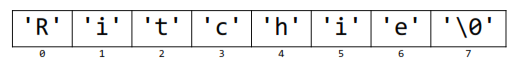
\includegraphics[width=0.6\textwidth]{pics/Zeichenkonstante.png}
 		\end{minipage}		
	\subsection{Operatoren und Begrenzer \verweiscpp{3.5}}
		Operatoren und Begrenzer sind einzelne Sonderzeichen bzw. Sequenzen von Sonderzeichen oder reservierten W�rter mit vordefinierter Bedeutung. Operatoren bestimmen Aktionen, die auf Programmobjekte ausgef�hrt werden k�nnen. Begrenzer wiederum trennen Symbole des Programmtexts voneinander.
	
	\subsection{Kommentare}
		\begin{minipage}[t]{13.5 cm}
			Kommentare sind Anmerkungen im Programmtext, die f�r den Leser bestimmt sind. Der Compiler ignoriert sie und entfernt sie vor dem �bersetzen des Programms in Maschinencode aus dem Quelltext.
		\end{minipage}
		\hspace*{1cm}
		\begin{minipage}[t]{4.5 cm}
			\lc{//} Einzeilige Kommentare \\
			\lc{/* */} Kommentare �ber \newline
			\phantom{} \ \ \ \ \ \ \ \ \ mehrere Zeilen
		\end{minipage}
		
	%\section{Einfache Deklarationen und Basisdatentypen \verweiscpp{4}}
	\subsection{Definition und Deklaration \verweiscpp{4.1}}
	Die Begriffe Deklaration und Definition werden oft synonym verwendet. Sie bezeichnen aber
	verschiedene Dinge: Eine Deklaration f�hrt einen oder mehrere Namen in einem Programm ein. Dem Compiler werden zwar mit dem Namen Informationen �ber einen Typ oder eine Funktion bekanntgegeben, es wird aber kein Programmcode erzeugt oder Speicherplatz f�r ein Objekt angelegt. Eine Definition wiederum vereinbart konkrete Objekte im Programm, also Variablen (inklusive deren Speicherplatz) oder ausf�hrbaren Code. Jede Definition ist damit zugleich eine Deklaration. 
	
	\begin{minipage}[t]{8 cm}
		\subsection{Variablendeklaration}
			\lstinputlisting[language=C++,tabsize=2]{code/variablendeklaration.cpp}
		
		\subsection{Variableninitialisierung}
			Um eine Variable zu initialisieren, gibt es mehrere M�glichkeiten:
			\lstinputlisting[language=C++,tabsize=2]{code/variableninit1.cpp}
			Eine Variable muss nicht sofort mit einem Wert initialisiert werden. Es ist auch m�glich, sie zun�chst nur zu definieren und ihr sp�ter einen Wert zuzuweisen.	
	\end{minipage}
	\hspace*{0.5 cm}
	\begin{minipage}[t]{10.5 cm}
		\subsection{Die One Definition Rule \verweiscpp{4.2}}
			Die One Definition Rule besagt vereinfacht dargestellt, dass ein Name genau einmal in einem Programm definiert sein darf. Es gibt jedoch einen Fall, bei dem diese Regel nicht verletzt wird und man trotzdem zwei Mal denselben Namen verwenden kann:
		
			\lstinputlisting[language=C++,tabsize=2]{code/one_definition_rule.cpp}
		
			Hier liegt keine Verletzung vor. \lc{A} ist in beiden Definitionen identisch und wird daher als eine einzelne Definition betrachtet. Ein Fehler l�ge dann vor, wenn die beiden Definitionen unterschiedlich w�ren.
			
		\subsection{Basisdatentypen \verweiscpp{4.3}}
			Basisdatentypen sind vordefinierte einfache Datentypen. Sie umfassen Wahrheitswerte (\lc{bool}), Zahlen (\lc{int}, \lc{short int}, \lc{long int}, \lc{float}, \lc{double}), Zeichen (\lc{char}, \lc{wchar\_t}) und den Typ "nichts"\phantom{} (\lc{void}).
	\end{minipage}
		
	\subsection{�bersicht �ber alle Standard-Datentypen \verweisc{5.2}}
		\begin{tabular}{|c|c|c|c|c|}
			\hline
				\textbf{Datentyp} & \textbf{Anzahl Bytes} & \textbf{Wertebereich (dezimal)} & Typ & Verwendung\\
			\hline
			\hline
				\lc{char} & 1 & $-128$ bis $+127$ & Ganzzahltyp & speichern eines Zeichens\\
			\hline
				\lc{unsigned char} & 1 & $0$ bis $+255$ & Ganzzahltyp & speichern eines Zeichens\\
			\hline
				\lc{signed char} & 1 & $-128$ bis $+127$ & Ganzzahltyp & speichern eines Zeichens\\
			\hline
			\hline
				\lc{int} & 4 (in der Regel) & $-2'147'483'648$ bis $+2'147'483'647$ & Ganzzahltyp & effizienteste Gr�sse\\
			\hline
				\lc{unsigned int} & 4 (in der Regel) & $0$ bis $+4'294'967'295$ & Ganzzahltyp & effizienteste Gr�sse\\
			\hline
			\hline
				\lc{short int} & 2 (in der Regel) & $-32'768$ bis $+32'767$ & Ganzzahltyp & kleine ganzzahlige Werte\\
			\hline
				\lc{unsigned short int} & 2 (in der Regel) & $0$ bis $+65'535$ & Ganzzahltyp & kleine ganzzahlige Werte\\
			\hline
			\hline
				\lc{long int} & 4 (in der Regel) & $-2'147'483'648$ bis $+2'147'483'647$ & Ganzzahltyp & grosse ganzzahlige Werte\\
			\hline
				\lc{unsigned long int} & 4 (in der Regel) & $0$ bis $+4'294'967'295$ & Ganzzahltyp & grosse ganzzahlige Werte\\
			\hline
			\hline
				\lc{float} & 4 (in der Regel) & $-3.4*10^{38}$ bis $+3.4*10^{38}$ & Gleitpunkttyp & Gleitpunktzahl\\
			\hline
				\lc{double} & 8 (in der Regel) & $-1.7*10^{308}$ bis $+1.7*10^{308}$ & Gleitpunkttyp & h�here Genauigkeit\\
			\hline
				\lc{long double} & 4 (in der Regel) & $-1.1*10^{4932}$ bis $+1.1*10^{4932}$ & Gleitpunkttyp & noch h�here Genauigkeit \\
			\hline
		\end{tabular}
		
		\subsubsection{Datentyp bool \verweiscpp{4.3.1}}
			Der Datentyp f�r Wahrheitswerte heisst in \lc{C++} \lc{bool}, was eine Abk�rzung f�r \lc{boolean} ist. Er kann nur zwei Zust�nde annehmen: \lc{true} (wahr) oder \lc{false} (falsch). Obwohl eigentlich 1 Bit ausreichen w�rde, hat \lc{bool} mindestens eine Gr�sse von einem Byte (also 8 Bit), denn 1 Byte ist die kleinste adressierbare Einheit und somit die Minimalgr�sse f�r jeden Datentyp. 
			
		\subsubsection{Datentyp void \verweiscpp{4.3.5}}
			\lc{void} ist ein spezieller Typ, der anzeigt, dass kein Wert vorhanden ist. Es ist nicht m�glich, ein Objekt vom Typ \lc{void} anzulegen. Vielmehr findet der Datentyp Anwendung bei der Deklaration von speziellen Zeigern, von denen nicht bekannt ist, auf welchen Typ sie verweisen, oder bei Funktionen, die keinen R�ckgabewert liefern.
			\vspace*{-0.01cm}\lstinputlisting[language=C++,tabsize=2]{code/void.cpp}

	\begin{minipage}[t]{9 cm}
		\subsection{Deklaration von Konstanten \verweiscpp{4.5}}
			Eine Konstante wird deklariert, indem vor dem eigentlichen Typ das Schl�sselwort \lc{const} notiert wird:
			\lstinputlisting[language=C++,tabsize=2]{code/const1.cpp}
			Wird versucht, w�hrend der Programmausf�hrung der Konstante \lc{val} einen Wert zuzuweisen, so f�hrt dies zu einem �bersetzungsfehler. \\
			Wichtig: Es g�be noch eine Variante mit \lc{\#define} (vorallem \lc{C}). Diese Variante sollte in \lc{C++} keinesfalls verwendet werden, da nur eine textuelle Ersetzung erfolgt! 
	\end{minipage}
	\hspace*{0.5 cm}
	\begin{minipage}[t]{8 cm}	
		\subsubsection{Zeichenkonstanten}
			\lstinputlisting[language=C++,tabsize=2]{code/const2.cpp}
		\subsubsection{Integerkonstanten}
			\lstinputlisting[language=C++,tabsize=2]{code/const3.cpp}
		\subsubsection{Fliesskommakonstanten}
			\lstinputlisting[language=C++,tabsize=2]{code/const4.cpp}
	\end{minipage}
	
	\subsection{Enumerations (Aufz�hlungstyp)}
	 	\begin{minipage}[t]{9 cm}
		 	\vspace*{-0.5cm}
		 	\lstinputlisting[language=C,tabsize=2]{code/enum1.c}
		 \end{minipage}
		 \hspace*{0.5 cm}
		 \begin{minipage}[t]{8 cm}
		 	\begin{compactitem}
		 		\item Aufz�hlungskonstanten haben einen konstanten ganzzahligen Wert.
		 		\item Die erste Konstante erh�lt den Wert \lc{0}, die zweite \lc{1}, etc.
		 		\item Werte k�nnen auch explizit zugewiesen werden
		 	\end{compactitem}
		\end{minipage}
		 		
		\subsubsection{Anonyme Enumerations}
			\begin{minipage}[t]{13 cm}
				\lc{enums} k�nnen auch verwendet werden, um ganzzahlige symbolische Konstanten zu definieren. Der \lc{enum} erh�lt dann keinen Namen, er wird nur dazu verwendet, die einzelnen Konstanten festzulegen. Bessere Alternative zu \lc{\#define} f�r ganzzahlige Konstanten!
			\end{minipage}
			\hspace*{0.5 cm}
			\begin{minipage}[t]{6 cm}
		 		\vspace*{-0.5cm}\lstinputlisting[language=C,tabsize=2]{code/enum2.c}
		 	\end{minipage}			
	
	\newpage
\section{Ausdr�cke und Operatoren}
	�hnlich wie mathematische Ausdr�cke stellen auch Ausdr�cke in \lc{C++} Berechnungen dar und bestehen aus Operanden und Operatoren. Die Auswertung jedes Ausdrucks liefert einen Wert, der sich aus der Verkn�pfung von Operanden durch Operatoren ergibt. 
	
	\subsection{Auswertungsreihenfolge}
		%Alle Ausdr�cke werden nach bestimmten Regeln ausgewertet. Massgeblich f�r die Art der Auswertung sind dabei Assoziativit�t und Priorit�t der Operatoren. \\
		\vspace*{-0.3cm}\begin{tabular}[t]{|p{1.5cm}|p{4cm}|p{8.5cm}|p{3.5cm}|}
			\hline	
				\textbf{Priorit�t} & \textbf{Operator} & \textbf{Beschreibung} & \textbf{Assoziativit�t} \\
			\hline
				1 & \lc{::} & Bereichsaufl�sung &  von links nach rechts\\
			\hline
				\multirow{5}{*}{2} & \lc{++ -\phantom{}-} & Suffix-/Postfix-Inkrement und -Dekrement & \multirow{5}{*}{von links nach rechts}\\
				& \lc{()} & Funktionsaufruf & \\
				& \lc{[]} & Arrayindizierung & \\
				& \lc{.} & Elementselektion einer Referenz & \\
				& \lc{->} & Elementselektion eines Zeigers & \\
			\hline
				\multirow{9}{*}{3} & \lc{++ -\phantom{}-} & Pr�fix-Inkrement und -Dekrement & \multirow{9}{*}{von rechts nach links} \\
				& \lc{+ -} & un�res plus und un�res Minus & \\
				& \lc{! \~} & logisches NOT und bitweises NOT & \\
				& \lc{(type)} & Typkonvertierung & \\
				& \lc{*} & Dereferenzierung & \\
				& \lc{\&} & Adresse von & \\
				& \lc{sizeof} & Typ-/Objektgr�sse & \\
				& \lc{new, new[]} & Reservierung Dynamischen Speichers & \\
				& \lc{delete, delete[]} & Freigabe Dynamischen Speichers & \\
			\hline
				4 & \lc{.* ->*} & Zeiger-auf-Element & von links nach rechts \\
			\hline
				5 & \lc{* / \%} & Multiplikation, Division und Rest & von links nach rechts \\
			\hline
				6 & \lc{+ -} & Addition und Subtraktion & von links nach rechts \\
			\hline
				7 & \lc{<\phantom{}< >\phantom{}>} & bitweise Rechts- und Linksverschiebung & von links nach rechts \\
			\hline
				\multirow{2}{*}{8} & \lc{< <=} & kleiner-als und kleiner-gleich & \multirow{2}{*}{von links nach rechts}\\
				& \lc{> >=} & gr�sser-als und gr�sser-gleich & \\
			\hline
				9 & \lc{== !=} & gleich und ungleich & von links nach rechts \\
			\hline
				10 & \lc{\&} & bitweises AND & von links nach rechts \\
			\hline
				11 & \lc{\textasciicircum} & bitweise XOR & von links nach rechts \\
			\hline
				12 & \lc{|} & bitweises OR & von links nach rechts \\
			\hline
				13 & \lc{\&\&} & logisches AND & von links nach rechts \\
			\hline
				14 & \lc{||} & logisches OR & von links nach rechts \\
			\hline
				\multirow{6}{*}{15} & \lc{?:} & bedingte Zuweisung & \multirow{6}{*}{von rechts nach links}\\
				& \lc{=} & einfache Zuweisung & \\
				& \lc{+= -=} & Zuweisung nach Addition/Subtraktion & \\
				& \lc{*= /= \%=} & Zuweisung nach Multiplikation, Division, Rest & \\
				& \lc{<\phantom{}<= >\phantom{}>=} & Zuweisung nach Links-, Rechtsverschiebung & \\
				& \lc{\&= \textasciicircum= |=} & Zuweisung nach bitweisem AND, XOR und OR & \\
			\hline
				16 & \lc{throw} & Ausnahme werfen & von rechts nach links \\
			\hline
				17 & \lc{,} & Komma (Sequenzoperator) & von links nach rechts \\
			\hline
		\end{tabular}

		\ \\ (Priorit�t 1 hat Vorrang vor allen anderen)
		
		\subsubsection{Assoziativit�t}
			Die Assoziativit�t gibt Auskunft �ber die Auswertungsreihenfolge der Operanden eines Ausdrucks. So wird zum Beispiel im Ausdruck \lc{p++} zuerst \lc{p} ausgewertet und dann die linke Seite des Operators \lc{++} (\lc{p}) erh�ht, w�hrend der Ausdruck \lc{++p} zuerst \lc{p} erh�ht und dann den Ausdruck auswertet.
			\lstinputlisting[language=C++,tabsize=2]{code/prio1.cpp}
			
		\subsubsection{Priorit�t}
			Die Priorit�t von Operatoren wiederum gibt an, in welcher Reihenfolge die verschiedenen Operanden eines Ausdrucks ausgewertet werden. Die multiplikativen Operatoren weisen zum Beispiel eine h�here Priorit�t als die additiven Operatoren auf.			
	

	%\section{Anweisungen}
	These der strukturierten Programmierung: 3 Anweisungen reichen aus, um jedes algorithmische Problem zu l�sen:
	\begin{compactitem}
  		\item Sequenz: Aufeinanderfolgende Anweisungen
  		\item Iteration: Die selbe Anweisung n-mal ausf�hren
  		\item Selektion: Anweisungen in Abh�ngigkeit einer Bedingung
  	\end{compactitem}
  	
	\subsection{Ausdrucksanweisungen}
    	\vspace*{-0.4cm}\begin{minipage}[t]{5 cm}
    		\subsubsection{Nullanweisung}  
   		 		Alleinstehender Strichpunkt   \\ 	
    			\lc{while(i < 5)\textbf{;}}    
    	\end{minipage}
    	\hspace*{0.5cm}
    	\begin{minipage}[t]{7 cm}
	    	\subsubsection{Zuweisung} 	    	
    			Einem Lvalue mittels \lc{=} , \lc{*=} , \lc{/=}, \lc{+=} oder \lc{-=} einen Wert zuweisen. \\   	
    			\lc{a=b=0 // entspricht a=(b=0)}
    	\end{minipage}	
   		\hspace*{0.5cm}
    	\begin{minipage}[t]{5 cm}
			\subsubsection{Funktionsaufruf} 
				\lc{getForFree(a, b);}
    	\end{minipage}
    	
	\subsection{Sprunganweisungen \verweisc{8.4}}
		Sprunganweisungen f�hren zu schlechtem Programmierstil und sollten nur in bestimmen F�llen eingesetzt werden, wie zum Bsp. \lc{break} bei \lc{switch}.
		\begin{compactitem}
			\item \lc{break}: \lc{do-while}-, \lc{while}-,  \lc{for}-Schleife und \lc{switch}-Anweisung abbrechen
			\item \lc{continue}: in den n�chsten Schleifendurchgang (Schleifenkopf) springen bei \lc{do-while}-, \lc{while}- und \lc{for}-Schleife 
			\item \lc{return}: aus Funktion an aufrufende Stelle zur�ckspringen mit R�ckgabe des Funktionswertes
			\item \lc{goto}: innerhalb einer Funktion an eine Marke (Label) springen
		\end{compactitem}
    	
	\begin{minipage}[t]{9 cm}
		\subsection{Sequenz \verweisc{8.1}}
			Die Sequenz ist eine zeitlich geordnete Abfolge von Anweisungen. \\
			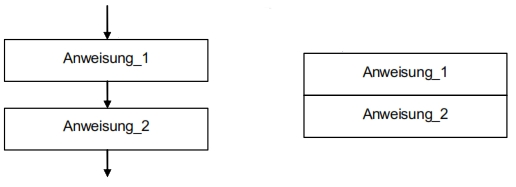
\includegraphics[width=1\textwidth]{pics/Sequenz.jpg}	
			
	\end{minipage}
	%
	\begin{minipage}[t]{9 cm}
			\subsubsection{Block}
				\begin{compactitem}
					\item Erfordert die Syntax genau eine Anweisung, so k�nnen dennoch mehrere Anweisungen geschrieben werden, wenn man sie in Form eines Blocks zusammenfasst.
					\item Ein Block wird mit geschweiften Klammern eingefasst. $\{ \dots \}$ Ein Block z�hlt syntaktisch als eine einzige Anweisung.
				\end{compactitem}
				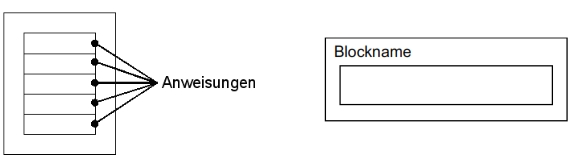
\includegraphics[width=1\textwidth]{pics/Block.jpg}
	\end{minipage}	   
    
	\subsection{Blockanweisungen}
		Anweisungen und Ausdr�cke innerhalb geschweifter Klammern. \\
    	\begin{minipage}[t]{9 cm}
        	\vspace*{-0.4cm}\lstinputlisting[language=C,tabsize=2]{code/block.c}
        \end{minipage}	
       	\hspace*{0.5cm}
        \begin{minipage}[t]{9 cm}
			Ausgabe: \\ \lc{x=15}  \lc{y=20} \\ \lc{x=5}  \lc{y=10} \\ kein Fehler, da der G�ltigkeitsbereich nur innerhalb des Blockes ist. Die ersten Variablen \lc{x} und \lc{y} werden im inneren Block lediglich �berdeckt.
        \end{minipage}
        
	\subsection{Selektionsanweisung \verweisc{8.2}}
		Von Selektion spricht man zum einen, wenn man eine Anweisung nur dann ausf�hren will, wenn eine bestimmte Bedingung zutrifft. Zum anderen m�chte man mit Selektionsanweisungen zwischen zwei M�glichkeiten (entweder/oder) bzw. zwischen mehreren M�glichkeiten genau eine ausw�hlen.
		
		\begin{minipage}[t]{5.5 cm}
			\subsubsection{Einfache Alternative}
				\lstinputlisting[language=C,tabsize=2]{code/strukturen_if_else.c}
		\end{minipage}
		%
		\begin{minipage}[t]{5.5 cm}
			\subsubsection{Bedingte Anweisung}
				\lstinputlisting[language=C,tabsize=2]{code/strukturen_if.c}
		\end{minipage}
		%
		\begin{minipage}[t]{7 cm}
			\subsubsection{Mehrfache Alternative - else if}
				\lstinputlisting[language=C,tabsize=2]{code/strukturen_else_if.c}
		\end{minipage}
		
		Wird innerhalb eines \lc{if} eine Variable deklariert, gilt sie bis zum Ende des \lc{if}.
		
		\subsubsection{Mehrfache Alternative - switch case}
			\begin{minipage}[t]{9 cm}
				
				\begin{compactitem}
					\item F�r eine Mehrfach-Selektion, d.h. eine Selektion unter mehreren Alternativen, kann die \lc{switch}-Anweisung verwendet werden, falls die Alternativen ganzzahligen Werten eines Ausdrucks von einem Integer-Typ entsprechen.
					\item Hat der Ausdruck der \lc{switch}-Anweisung den gleichen Wert wie einer der konstanten Ausdr�cke der \lc{case}-Marken, wird die Ausf�hrung des Programms mit der Anweisung hinter dieser \lc{case}-Marke weitergef�hrt.
					\item Stimmt keiner der konstanten Ausdr�cke mit dem \lc{switch}-Ausdruck �berein, wird zu \lc{default} gesprungen.
				\end{compactitem}							
			\end{minipage}
			\hspace*{1cm}
			\begin{minipage}[t]{9 cm}
				\vspace*{-0.5cm}
				\lstinputlisting[language=C,tabsize=2]{code/strukturen_switch.c}
			\end{minipage}
			
	\subsection{Iteration \verweisc{8.3}}
		\begin{minipage}[t]{4 cm}
			\vspace*{-0.4cm}\subsubsection{While}
				\vspace*{-0.4cm}\lstinputlisting[language=C,tabsize=2]{code/strukturen_while.c}			
		\end{minipage}
		\begin{minipage}[t]{14 cm}
			\vspace*{0.05cm}Schleifenrumpf wird ausgef�hrt solange Bedingung \lc{true} ergibt. \lc{do..while} und \lc{for} k�nnen grunds�tzlich aus \lc{while} gebaut werden.
		\end{minipage}
		
		\begin{minipage}[t]{10 cm}
			\subsubsection{For-Schleife}
				\vspace*{-0.4cm}\lstinputlisting[language=C,tabsize=2]{code/strukturen_for.c}
		\end{minipage}
		\begin{minipage}[t]{8 cm}
			\vspace*{0.45cm}Laufvariablen lokal deklarieren: \\\lc{for(int i=0; i<100; ++i)} \\Damit gilt sie nur innerhalb der Schleife.
		\end{minipage}

		\begin{minipage}[t]{4 cm}
			\subsubsection{Do-While}
				\vspace*{-0.4cm}\lstinputlisting[language=C,tabsize=2]{code/strukturen_dowhile.c}
		\end{minipage}
		\begin{minipage}[t]{14 cm}
			\vspace*{0.45cm}Schleifenrumpf wird mind. einmal ausgef�hrt und wiederholt falls Bedingung \lc{true} ergibt.
		\end{minipage}
		
		\subsubsection{Endlosschleife}
			\begin{minipage}[c]{3 cm}
				\vspace*{-0.4cm}\lstinputlisting[language=C,tabsize=2]{code/strukturen_endlos_for.c}
			\end{minipage}
			%
			\begin{minipage}[c]{3 cm}
				\vspace*{-0.4cm}\lstinputlisting[language=C,tabsize=2]{code/strukturen_endlos_while.c}
			\end{minipage}
		
		\subsubsection{Wann wird welche Schleife eingesetzt?}
			\begin{compactitem}
				\item For-Schleife: Bei Z�hlschleifen, d.h. wenn die Anzahl Durchl�ufe (kann auch variabel sein) im
				voraus feststeht.
				\item Do-While-Schleife: Wenn es keine Z�hlschleife ist, und die Schleife muss mindestens einmal
				durchlaufen werden
				\item While-Schleife: In allen anderen F�llen
			\end{compactitem}        

	\newpage
\section{Funktionen}
	Im Vergleich zu \lc{C} funktionieren Funktionen in \lc{C++}	genau gleich, zus�tzlich gibt es aber einige neue, n�tzliche Eigenschaften:
	\begin{compactitem}
		\begin{multicols}{2}
			\item Vorbelegung von Parametern (Default-Argumente)
			\item �berladen von Fuktionen (Overloading)
			\item Operatorfunktionen
			\item inline-Funktionen
		\end{multicols}
	\end{compactitem}	
	\subsection{�berladene Funktionen}
		\begin{minipage}[t]{13cm}
			\begin{compactitem}
				\item Die Identifikation einer Funktion erfolgt �ber die Signatur, nicht nur �ber den Namen. Die Signatur besteht aus dem Namen der Funktion plus der Parameterliste (Reihenfolge, Anzahl, Typ). Der Returntyp wird nicht ber�cksichtigt.
				\item Der Name der Funktionen ist identisch.
				\item Die Implementation muss f�r jede �berladene Funktion separat erfolgen.
				\item Overloading sollte zur�ckhaltend eingesetzt werden. Wenn m�glich sind Default-Argumente vorzuziehen.
			\end{compactitem}
		\end{minipage}
		\hspace*{0.5cm}
		\begin{minipage}[t]{5cm}
			\vspace*{-0.3cm}
			\lstinputlisting{code/overloading.cpp}
		\end{minipage}
	
	\subsection{Vorbelegte Parameter}
		\begin{minipage}[t]{8 cm}
			\begin{compactitem}
				\item Parametern k�nnen im Funktionsprototypen Defaultwerte	zugewiesen werden. 
				\item Beim Funktionsaufruf k�nnen (aber m�ssen nicht) die Parameter mit Defaultwerten weggelassen	werden.
				\item Achtung: Hinter (rechts von) einem Default-Argument darf kein nicht vorbelegter Parameter mehr folgen!
			\end{compactitem}
		\end{minipage}
		\hspace*{0.5cm}
		\begin{minipage}[t]{10 cm}	
			\vspace*{-0.3cm}
			\lstinputlisting[language=C++,tabsize=2]{code/default_parameter.cpp}
		\end{minipage}
					
	\subsection{$inline$-Funktionen vs. $C$-Makros}
		\begin{minipage}[t]{8 cm}
			\subsubsection{$C$-Makros}
				\begin{compactitem}
					\item $C$-Makros werden definiert mit $\#define$.
					\item $C$-Makros bewirken eine reine Textersetzung ohne jegliche Typenpr�fung.
					\item Bei Nebeneffekten (welche zwar vermieden werden sollten) verhalten sich Makros nicht wie beabsichtigt.
					\item $C$-Makros l�sen zwar das Problem mit dem Overhead, sind aber sehr unsicher.				
				\end{compactitem}
				\lstinputlisting[language=C,tabsize=2]{code/c_makro.c}
			\end{minipage}
			\hspace*{0.5cm}
			\begin{minipage}[t]{10 cm}	
				\subsubsection{$inline$-Funktionen}
					\begin{compactitem}
						\item L�sen das Overhead-Problem.
						\item Textersetzung mit Typenpr�fung.
						\item Einsetzen wenn der Codeumfang der Funktion sehr klein ist und die Funktion h�ufig aufgerufen wird (z.B. in Schleifen).
						\item Rekursive Funktionen und Funktionen, auf die mit einem Funktionspointer gezeigt wird, werden nicht ge-$inlined$.
					\end{compactitem}
					\lstinputlisting[language=C++,tabsize=2]{code/inline.cpp}
			\end{minipage}	
		

	
	
	
	\newpage
\section{H�here und strukturierte Datentypen}
	\begin{minipage}[t]{6 cm} 		
  		\subsection{Pointer}
  			Pointer sind in \lc{C++} zu 99\% wie in \lc{C}. \\
		\subsubsection{Null-Pointer}
			Ab \lc{C++11} gibt es einen vordefinierten Wert f�r den Nullpointer: \lc{nullptr}
			\vspace*{-0.2cm}\lstinputlisting{code/pointer_null.c}
	\end{minipage}	
	\hspace*{0.5cm}
	\begin{minipage}[t]{12 cm}
		\subsubsection{$void$-Pointer}
			\begin{compactitem}
				\item Wenn bei der Definition des Pointers der Typ der Variable, auf die der Pointer zeigen soll, noch nicht feststeht, wird ein Pointer auf den Typ \lc{void} vereinbart.
				\item Ein Pointer auf \lc{void} umgeht die Typenpr�fung des Compilers. Er kann ohne \lc{typecast} einem typisierten Pointer zugewiesen werden aber er kann keine Zuweisung von einem typisierten Pointer erhalten (in \lc{C} erlaubt).
				\item Jeder Pointer kann durch Zuweisung in den Typ \lc{void*} und zur�ck umgewandelt werden, ohne dass Informationen verloren gehen.
			\end{compactitem}
 	\end{minipage}
 	       
	\subsubsection{Pointer auf Funktionen}
		\begin{minipage}[t]{10 cm}
			\vspace*{-0.5cm}\lstinputlisting{code/pointer_funktion.c}
		\end{minipage}
		\hspace*{0.5cm}
		\begin{minipage}[t]{8 cm}
			\vspace*{-0.6cm}
			\textbf{Vereinbarung eines Pointers}
				\lstinputlisting{code/pointer_funktion_vereinbarung.c}
				$ptr$ ist hier ein pointer auf eine Funktion mit R�ckgabewert vom Typ $int$ und einem �bergabeparameter vom Typ $char$. Die Klammern m�ssen unbedingt gesetzt werden. \\
			
			\textbf{Zuweisung einer Funktion}
				\lstinputlisting{code/pointer_funktion_zuweisung.c} \ \\
				
			\vspace*{-0.7cm}\textbf{Aufruf einer Funktion}
				\lstinputlisting{code/pointer_funktion_aufruf.c}
		\end{minipage}
       
	\subsubsection{const bei Pointern}
		\vspace*{-0.3cm}
		\begin{minipage}[t]{5 cm}
			\paragraph{konstanter String}
			\vspace{-0.5cm}
			\lstinputlisting{code/const_pointer_1.c}
		\end{minipage}
		\hspace*{0.5cm}
		\begin{minipage}[t]{5 cm}
			\paragraph{konstanter Pointer}
			\vspace{-0.5cm}
				\lstinputlisting{code/const_pointer_2.c}
		\end{minipage} 
		\hspace*{0.5cm}
		\begin{minipage}[t]{7.5 cm}					
			\paragraph{konst. Pointer auf konst. String}
				\vspace{-0.5cm}
				\lstinputlisting{code/const_pointer_3.c}
		\end{minipage} 

\phantom{}

	\subsection{Referenzen}
		\begin{compactitem}
			\item Referenzen sind alternative Namen oder Alias f�r ein Objekt
			\item Beim Pointer m�chte man eine Adresse, eine Referenz kann auch auf Register verweisen
			\item Wenn immer m�glich sollten Referenzen verwendet werden, weil sicherer
		\end{compactitem}
		\begin{minipage}[t]{10.5 cm}
	  		\vspace*{-0.3cm}\lstinputlisting{code/ref1.c}
	  	\end{minipage}				
   
	\subsection{Pointer und Referenzen als R�ckgabewert und Parameter�bergabe}
  		Bei Variablen�bergabe (call by value) werden Kopien �bergeben, welche nicht ver�ndert werden k�nnen.\\
  		Bei Referenz�bergabe (call by reference) kann die Subroutine die Werte bleibend ver�ndern. \\
  		\textbf{Objekte einer Klasse und Strukturvariablen sollen immer by reference �bergeben werden!} \\
  		\begin{minipage}[t]{5.5 cm}
  			\subsubsection{call by reference}
   				\lstinputlisting{code/swap.c} 
   		\end{minipage}
   		\hspace*{0.5cm}
    	\begin{minipage}[t]{5.5 cm}
      			\vspace*{0.77cm} \lstinputlisting{code/swap2.c} 
      	\end{minipage}
      	\hspace*{0.5cm}
      	\begin{minipage}[t]{6 cm}
      		\subsubsection{call by value}
      	      	\lstinputlisting{code/swap3.c} 
      	\end{minipage}
      \\
      
    \subsection{Dynamische Speicherverwaltung}
    	\begin{minipage}[t]{9 cm}
    		\subsubsection{pro Memoria: Variablen}
	    		\begin{compactitem}
	    			\item erleichtern u.a. den Zugriff auf Speicherstellen (anstelle Adressen)
	    			\item M�ssen zur Entwicklungszeit im Code definiert werden
	    			\item Der Speicher einer Variable wird automatisch freigegeben, sobald die Variable nicht mehr g�ltig ist.
	    		\end{compactitem}  	
	    	\subsubsection{Dynamische Speicherverwaltung}
		    	\begin{compactitem}
		    		\item Speicher kann zur Laufzeit (dynamisch) vom System angefordert (alloziert) werden
		    		\begin{compactitem} \item Operator: $new$ (in $C$: Funktion $malloc()$) \end{compactitem}
		    		\item Dynamisch allozierter Speicher muss wieder explizit freigegeben werden
		    		\begin{compactitem} \item Operator: $delete$ (in $C$: Funktion $free()$) \end{compactitem}
		    		\item Dynamischer Speicher wird nicht auf dem Stack angelegt, sondern auf dem {\bf Heap}
		    		\item Auf Dynamisch allozierter Speicher kann {\bf nur} �ber Pointer zugegriffen werden
		    	\end{compactitem}
	    \end{minipage}
		\hspace*{0.5cm}
		\begin{minipage}[t]{9 cm}
			\subsubsection{Syntax}
			\vspace*{-0.3cm}
			\lstinputlisting{code/speicherverw.c}
		\end{minipage}
	
	\subsubsection{Vorsichtsmassnahmen}
		\begin{compactitem}
			\item Beim Anwenden des delete-Operator auf einen bereits freigegebenen Speicherbereich, kann Probleme verursachen.
			\item Oft wird deshalb ein Pointer nach der $delete$-Operation auf 0 (bzw. $nullptr$) gesetzt.
		\end{compactitem}
	
	\subsubsection{Memory Leak, Garbage Collection}
	\begin{compactitem}
		\item {\bf Memory Leak} = Speicher, der nicht freigegeben wurde oder auf welchen der Zugriff verloren ging, belegt
		aber weiterhin Platz im Speicher. (wie ein Leck)
		\item In einigen Programmiersprachen (wie z.B. Java) gibt es einen sogenannten {\bf Garbage Collector}, welcher dieser Speicher automatisch freigibt.
		\item In C++ gibt es keinen Garbage Collector. Der Programmierer ist selber daf�r verantwortlich.
	\end{compactitem}
 		
	\subsubsection{Dynamische Allozierung von Arrays}
		\begin{minipage}[t]{7 cm} 
			\begin{compactitem}
				\item mit \lc{new[]} kann dynamischer Speicher f�r ein Array alloziert werden.
				\item Zugriff erfolgt wie bei statischen Arrays.
				\item Mit \lc{delete[]} k�nnen dynamisch allozierte Arrays wieder explizit freigegeben werden.
			\end{compactitem}
		\end{minipage}
		\hspace*{0.5cm}
		\begin{minipage}[t]{11 cm}
			\vspace*{-0.3cm}
			\lstinputlisting{code/vec2.c}
		\end{minipage}
	
	\subsubsection{Dynamische Allozierung von Matrizen}
		\paragraph{Variante 1}
			\begin{compactitem}
				\item m*n-Matrix als eindimensionaler Array der Gr�sse (m*n)
				\item Zugriff nur �ber Pointer:
			\end{compactitem}
			\lstinputlisting{code/matrix1.cpp}
    	\paragraph{Variante 2}
    		\begin{compactitem}
				\item Ein Array der Gr�sse m und dem Typ Array
				\item Auf ein Matrixelement kann somit �ber Arrayindizes zugegriffen werden:
    		\end{compactitem}
    		\lstinputlisting{code/matrix2.cpp}
    		\begin{minipage}[t]{9 cm}
    			\vspace*{-2.5 cm}
    			\lstinputlisting{code/matrix3.cpp}
    		\end{minipage}
    		\hspace*{0.5cm}
    		\begin{minipage}[t]{9 cm}
    			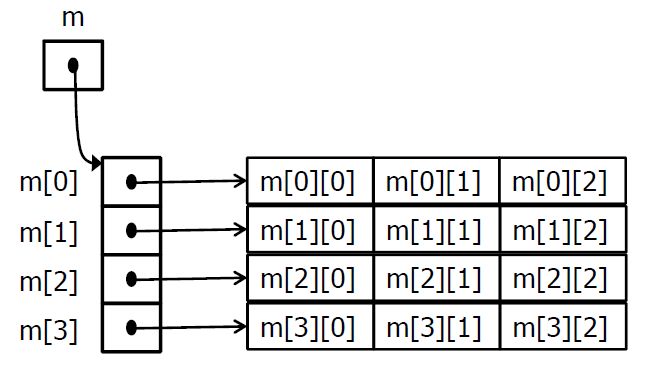
\includegraphics[width=5cm]{pics/matrix.png}
    		\end{minipage}
    		\begin{compactitem}
    			\item Jedes \lc{m[i]} ist ein Pointer auf ein Array mit 3 Elementen vom Typ \lc{double}.
    			\item \lc{m[i]} selbst ist vom Typ \lc{double*}.
    			\item der Speicher von Matrizen wird wie folgt freigegeben (zuerst jede Zeile dann Array mit \lc{double*}):
			\end{compactitem}
			\lstinputlisting{code/matrixDel.cpp}
		\paragraph{Vor- und Nachteile Variante 2}
			\begin{compactitem}
				\vspace*{-0.3cm}
				\item Nur mit der Variante 2 kann �ber Arrayindizes zugegriffen werden
				\item Die einzelnen Zeilen liegen m�gicherweise nicht auf aufeinanderfolgenden Speicherstellen
				\item Der Zugriff ist effizienter, obwohl man zus�tzliche Pointer ben�tigt
			\end{compactitem}
			
	\subsection{Structs}
		\begin{minipage}[t]{5 cm}
			\begin{compactitem}
				\item Grunds�tlich wie in $C$
				\item $typedef$ braucht es nicht
			\end{compactitem}	
		\end{minipage}
		\hspace*{0.5cm}
		\begin{minipage}[t]{5 cm}
			{\bf Beispiel in $C$:}
			\lstinputlisting{code/structC.c}
		\end{minipage}  
		\hspace*{0.5cm}
		\begin{minipage}[t]{5 cm}
		{\bf Beispiel in $CPP$:}
		\lstinputlisting{code/structCpp.cpp}
		\end{minipage} 
		


	\newpage
\section{G�ltigkeitsbereiche, Namensr�ume und Sichtbarkeit}
	\subsection{Namensr�ume}
		\begin{minipage}[t]{4.5 cm}
			\lstinputlisting{code/namespace.cpp}
		\end{minipage}
		\begin{minipage}[t]{14.5 cm}
			Namensr�ume sind G�ltigkeitsbereiche, in denen beliebige Bezeichner (Variablen, Klassen, Funktionen, andere Namensr�ume, Typen, etc.) deklariert werden k�nnen.
			\begin{compactitem}
				\item Ein Namensraum kann deklariert werden. Alle enthaltenen Objekte werden diesem Namensraum zugeordnet. Auf Bezeichner eines Namensraumes kann mit dem Scope Operator \lc{::} zugegriffen werden.
				\item Einem Namensraum kann ein so genannter Alias zugeordnet werden, �ber den er angesprochen wird. \\
				\lc{namespace FBSSLIB = Financial\_Branch\_and\_System\_Service\_Library;}
				\item Eine so genannte \lc{Using}-Deklaration erlaubt den direkten Zugriff auf einen Bezeichner eines Namensraumes. \\
				\lc{using MyLib1::foo;} \\
				\lc{foo();}
				\item Mit einer so genannten \lc{Using}-Direktive kann auf alle Bezeichner eines Namensraums direkt zugegriffen werden. \\
				\lc{using namespace MyLib1;} \\
				\lc{foo();}			
			\end{compactitem}
		\end{minipage}
		\subsubsection{namenlose Namensr�ume}
			\begin{minipage}[t]{4cm}
				Anstelle von \lc{static} in $C$
			\end{minipage}
			\hspace*{0.5cm}
			\begin{minipage}[t]{3cm}
				\vspace*{-0.2cm}
				\lstinputlisting{code/namelessNamespace.cpp}
			\end{minipage}
			
	\subsection{Deklarationen}
		\subsubsection{Speicherklassenattribute}
			\begin{compactitem}
				\item \lc{auto}: gilt als Standard wenn nichts anderes steht. G�ltigkeitsbereich der \lc{auto} Variablen ist innerhalb des Blockes in dem sie deklariert wurde.
				\item \lc{register}: Hinweis an den Compiler m�glichst die Variable in einem Register abzulegen.
				\item \lc{static}: Variablen leben von ihrer Deklaration bis zum Programmende. Geeignet um zum Bsp. Funktionsaufrufe zu z�hlen anstatt mit globaler Variable.
				\item \lc{extern}: Zugriff auf eine \lc{static} Variable in einem anderen File, welches zu einem gesamten Programm gelinkt wurde.
				\item \lc{mutable}: Klassenelemente mit \lc{const} oder \lc{static} Attributen k�nnen nachtr�glich ver�ndert werden.
			\end{compactitem}
	
		\subsubsection{Typqualifikatoren}
		\begin{compactitem}
			\item \lc{const}: Objekte d�rfen nicht ver�ndert werden. RValues.
			\item \lc{volatile}: Objekte werden evtl. von Aussen im Programmverlauf ver�ndert, und d�rfen daher vom Compiler nicht zu Optimierungszwecken zwischengespeichert werden. Sie werden immer aus dem Hauptspeicher eingelesen.\\
			Verlangsamt das Programm, sollte daher gezielt eingesetzt werden.
		\end{compactitem}
		
		\subsubsection{typedef}
			\begin{minipage}[t]{10 cm}
				\vspace*{-0.3cm}\lstinputlisting[language=C,tabsize=2]{code/typedef.c}
			\end{minipage}
			\begin{minipage}[t]{9 cm}
				\vspace*{-0.35cm}
				Das Schl�sselwort \lc{typedef} erm�glicht die Einf�hrung neuer Bezeichner, die dann im Programm anstelle von anderen Typen verwendet werden k�nnen. \lc{typedef} f�hrt allerdings keine neuen Typen, sondern Synonyme f�r einen existierenden Datentyp ein. Es ist also mehr oder weniger eine Textersetzung.
			\end{minipage}
		 
	\newpage\subsection{Type-cast}
		\subsubsection{implizite-Typumwandlung}
			Ausdr�cke werden bei einer Zuweisung automatisch in den erwarteten Typ umgewandelt.
			\lstinputlisting{code/typecast.c}
	
	\begin{minipage}[t]{4 cm}
		\subsubsection{$C$-Stil}
			\lstinputlisting{code/typecast2.c}
	\end{minipage}
	\hspace*{0.5cm}
	\begin{minipage}[t]{4cm}
		\subsubsection{Funktions-Stil}
			\lstinputlisting{code/typecast3.c}
	\end{minipage}
	\hspace*{0.5cm}
	\begin{minipage}[t]{9.5cm}
		\vspace*{0.1cm}
		{\bfseries Achtung:} Den \lc{C}- und Funktions-Stil sollte in \lc{C++} nicht verwendet werden, da daraus der Grund f�r die Typumwandlung nicht erkannt wird und der Compiler keine Pr�fung durchf�hrt. Deshalb stellt \lc{C++} die folgenden spezifischen und sichereren Typumwandlungen zur Verf�gung.
	\end{minipage}
	
	\subsubsection{Neu in $C++$:}
		\paragraph{\lc{const\_cast}}
			Ausschliesslich bei der Entfernung des \lc{const}-Qualifikators.\\
			Syntax:
			\lstinputlisting{code/constcast.c}
			Beispiel:
			\lstinputlisting{code/constcast_bsp.cpp}
		\paragraph{\lc{static\_cast}}
			Umwandeln eines Klassenobjekt in ein Objekt seiner Basisklasse. Syntax ist analog zu \lc{const\_cast}.\\
			Beispiel:
			\lstinputlisting{code/staticcast.cpp}
		\paragraph{\lc{dynamic\_cast}}	
			Umwandlung von Polymorphen Objekten im Zusammenhang mit dem Typsystem von C++.\\
			Beispiel:
			\lstinputlisting{code/dynamiccast.cpp}
		\paragraph{\lc{reinterpret\_cast}}
			Neue Interpretation der zugrunde liegenden Bitkette.\\
			Beispiel:
			\lstinputlisting{code/reinterpret_cast.cpp}
		
		
		
	\newpage
\section{Module und Datenkapseln}
	Modul = Unit	\hspace*{2cm}	Modultest = Unittest \\
	\begin{minipage}[t]{9 cm}
		\subsection{Motivation}
		\begin{compactitem}
			\item {\bf Arbeitsteilung:} Grosse Programme werden von mehreren Personen entwickelt.
			\item {\bf Effizienz:} Eine �bersetzungseinheit (Datei) muss bei jeder �nderung neu �bersetzt werden (je gr�sser die Datei desto langsamer die �bersetzung)
			\item {\bf Strukturierung:} Ein grosses Programm in mehrere vern�nftige Teile (Baugruppen, Units) aufteilen (Divide and conquer) 

		\end{compactitem}
	\end{minipage}
	%\hspace*{0.5cm}
	\begin{minipage}[t]{9 cm}
		\subsection{Ziele der Modularisierung}
			\begin{compactitem}
				\item Klare, m�glichst schlanke Schnittstellen definieren
				\item Units so bilden, das Zusammengeh�rendes in einer Unit isoliert wird (Koh�sion soll hoch sein)
				\item Schnittstellen zwischen den Units sollen klein sein (Kopplung soll klein sein)
				\item Abh�ngigkeiten unter den Units sollen eine Hierarchie bilden, zirkul�re (gegenseitige) Abh�ngigkeiten m�ssen vermieden werden
			\end{compactitem}
	\end{minipage}

	\subsection{Vom Modul zur Datenkapsel}
		Eigenschaften einer Unit (eines Moduls):
		\begin{compactitem}	
			\item realisiert eine in sich abgeschlossene Aufgabe
			\item kommuniziert �ber ihre Schnittstelle mit der Umgebung
			\item kann ohne Kenntnisse ihres inneren Verhaltens in ein Gesamtsystem integriert werden (include Header)
			\item ihre Korrektheit kann ohne Kenntnis ihrer Einbettung in einem Gesamtsystem nachgewiesen werden (mittels Unittest)
			\item \textbf{Die Datenkapsel fordert nun zus�tzlich, dass auf die Daten nicht direkt zugegriffen werden darf, sondern nur �ber Zugriffsfunktionen.}
		\end{compactitem}
		Die Schnittstelle beschreibt, was das Modul zur Verf�gung stellt, verbirgt dabei wie das Verhalten konkret realisiert ist (Geheimnisprinzip, Information Hiding). Der User der Unit darf keine Annahme �ber den inneren Aufbau machen. Der Entwickler der Unit kann deren inneren Aufbau ver�ndern, solange die Schnittstelle dadurch nicht �ndert. \\

	\subsection{Unitkonzept / Module und Datenkapseln in C++}
		\begin{minipage}[t]{10 cm}
		    \begin{compactitem}
		    	\vspace*{-2.5cm}
			  	\item Interface definiert die Schnittstelle, d.h. die Deklarationen wie Funktionsprototypen, etc. (Schaufenster)
			  	\item Implementation: in diesem Teil sind die Unterprogramme definiert, d.h. auscodiert (Werkstatt)
				 \item Das Interface wird in einer Headerdatei (\lc{*.h}) beschrieben, die Implementation liegt in einer \lc{*.cpp}- Datei
			\end{compactitem}
		\end{minipage}
		\hspace*{0.5cm}
		\begin{minipage}[t]{8cm}
			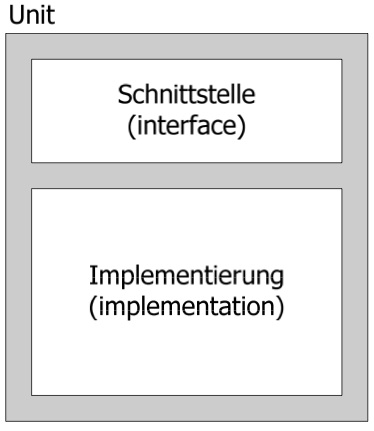
\includegraphics[width=0.28\textwidth]{pics/unit.jpg}
		\end{minipage}

    \subsection{Die Schnittstellendatei}
		\begin{minipage}[t]{10 cm}
			 Jede \lc{.h}-Datei enth�lt als erste Anweisungsfolge einen Include-Guard welcher Mehrfacheinf�gen verhindert. Der Syntax lautet:
			 \lstinputlisting[language=C,tabsize=2]{code/includeguard.c}
			 Deklarationsreihenfolge in Headerdatei (*.h)
			\begin{compactenum}
				\item Dateikommentar
				\item \lc{\#include} der verwendeten System-Header (\lc{iostream}, etc.) \newline
				      \lc{\#include <...>}
				\item \lc{\#include} der projektbezogenen Header (\lc{\#include "..."})
				\item Konstantendefinitionen
				\item \lc{typedef}s und Definition von Strukturen
				\item Allenfalls extern-Deklaration von globalen Variablen
				\item Funktionsprototypen, inkl. Kommentare der Schnittstelle, bzw. Klassendeklarationen
			\end{compactenum}
			\begin{compactitem}
				\item {\bf Achtung:} kein \lc{using namespace} in Headerdateien!
			\end{compactitem}
		\end{minipage}	
		\hspace*{0.5cm}	
     	\begin{minipage}[t]{8 cm}
     		\vspace*{-0.9cm}
			\subsection{Die Implementierungsdatei}
				Deklarationsreihenfolge in Implementierungsdatei (\lc{*.cpp})
				\begin{compactenum}
			 		\item Dateikommentar
					\item \lc{\#include} der verwendeten System-Header (\lc{iostream}, etc.)
					      \lc{\#include <...>}
					\item \lc{\#include} der projektbezogenen Header (\lc{\#include "..."})
					\item Verwendung von \lc{using namespace}
					\item allenfalls globale Variablen und statische Variablen
					\item Pr�prozessor-Direktiven
					\item Funktionsprototypen von lokalen, internen Funktionen
					\item Definition von Funktionen und Klassen (Kommentare aus Headerdatei nicht wiederholen!) 
				\end{compactenum}
		\end{minipage}
		
		\subsection{Buildprozess / Makefile}
			\begin{minipage}[t]{12 cm}
			    Der Buildprozess erstellt aus den einzelnen Dateien einen ausf�hrbaren Code. Dazu werden zuerst alle \lc{*.cpp}-Files compiliert.
			    Die daraus entstandenen Objektdateien m�ssen anschliessend gelinkt und somit zu einer ausf�hrbaren Datei zusammengesetzt. Die Eingabe in der Konsole sieht wie folgt aus:
			    \lstinputlisting[language=C,tabsize=2]{code/compileUnit.c}
				Es w�re m�hsam, wenn diese Befehle jedesmal neu eingetippt werden m�ssten. Deshalb wird in der Praxis oft ein Buildtool eingesetzt, z.B. \lc{make}.
			\end{minipage}
			\hspace*{0.5cm}
			\begin{minipage}[t]{6.5 cm}
				Abh�ngigkeitsliste gem�ss  UML-Notation: \\
				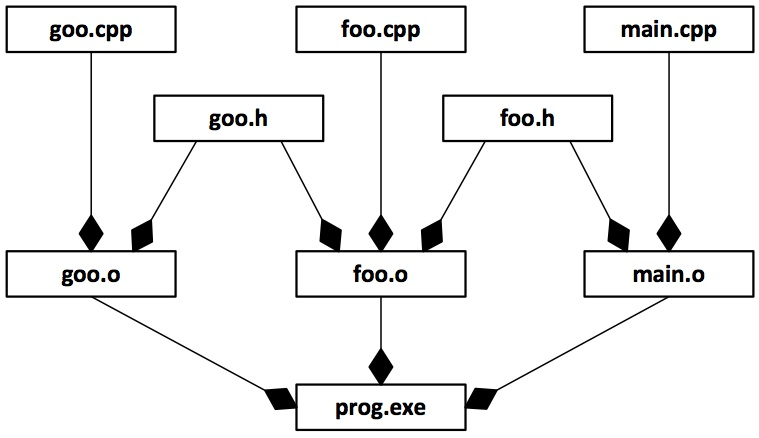
\includegraphics[width=0.85\textwidth]{pics/abhaengigkeitUML.jpg}		    
			\end{minipage}
			
			\subsubsection{Make-File}
				\begin{minipage}[c]{10 cm}
					\vspace*{-3.2cm}\begin{compactitem}	
						\item In einem \lc{make}-File k�nnen Abh�ngigkeiten definiert werden
						\item  Wenn eine Datei ge�ndert wurde, dann werden alle Operationen ausgef�hrt mit den Dateien, welche von dieser ge�nderten Datei abh�ngen
						\item Der Befehl (\lc{g++}) wird z.B. nur dann ausgef�hrt, wenn sich an den Dateien, zu denen eine Abh�ngigkeit besteht, etwas ge�ndert hat
					\end{compactitem}
				\end{minipage}
				\hspace*{0.5cm}
				\begin{minipage}[c]{8.5 cm}
					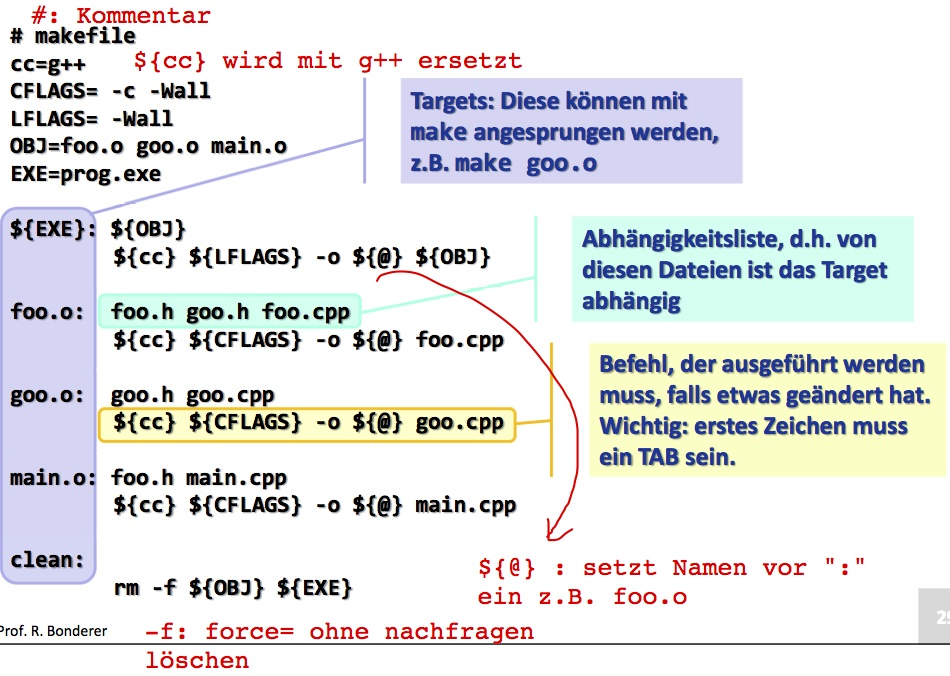
\includegraphics[width=1\textwidth]{pics/makefile.jpg}	
				\end{minipage}			     										
	
	\newpage
\section{Klassenkonzept}
	\subsection{Begriff der Klasse}
		\begin{compactitem}
			\item Eine Klasse ist eine Struktur (eine Struktur besteht nur aus Daten), die mit den 	Funktionen, welche auf diesen Daten arbeiten, erweitert wurde.
			\item Eine Klasse ist also eine Struktur, welche die Daten und die Funktionen auf diesen Daten in ein syntaktisches Konstrukt packt.
			\item Die Klasse ist die Umsetzung der Datenkapsel.
			\item Eine Klassendeklaration ist eine Typendefinition. Die Variablen einer Klasse
			werden als Objekte bezeichnet.
		\end{compactitem}
	\begin{minipage}[t]{10cm}
		\subsection{UML ist...}
			\begin{compactitem}
				\item ... die Abk�rzung f�r {\bf U}nified {\bf M}odelling {\bf L}anguage
				\item ... eine graphische Modellierungssprache
				\item ... ein fortlaufendes (objektorientiertes) Modellierungskonzept f�r alle Software-Entwicklungsphasen (Ziel der UML)
				\item ... der Standard f�r Softwaremodellierung
				\item ... (programmier-)sprachunabh�ngig
				\item ... {\bf kein} Softwareprozess-Modell
				\item ... {\bf kein} Lebenszyklusmodell
				\item ... {\bf keine} Programmiersprache
				\item ... {\bf nicht} ohne Redundanz (es gibt oft mehrere M�glichkeiten, etwas zu modellieren)
				\item ... {\bf kein} Softwaretool
			\end{compactitem}
	\end{minipage}	
	\hspace*{0.5cm}
	\begin{minipage}[t]{8 cm}
		\subsection{UML-Notation einer Klasse}
			\begin{center}
				\begin{tikzpicture}
					\begin{class}[text width=4cm]{ClassName}{0 ,0}
						\attribute {-attribute1: int = 0}
						\attribute {-attribute2: int = 0}
						\operation {+method1()}
						\operation {+method2()}
					\end{class}
				\end{tikzpicture}
			\end{center}
			\begin{compactitem}
				\item Eine Klasse ist der Bauplan f�r Objekte.
				\item Eine Klasse besteht aus Daten (Attribute) und den Funktionen (Methoden) auf diesen Daten.
				\item Sichtbarkeit: 
				\begin{compactitem}
					\item \lc{+} : \lc{public}
					\item \lc{-} : \lc{private}
					\item \lc{\#} : \lc{protected}
				\end{compactitem}
			\end{compactitem}
	\end{minipage} \\
	
	\begin{minipage}[t]{8 cm}	
		\subsection{�blicher Aufbau einer Klassensyntax}
			\lstinputlisting{code/klassenschnittstelle.cpp} 
	\end{minipage}
	\hspace*{0.5cm}
	\begin{minipage}[t]{10 cm}		
			\subsubsection{Zugriffsschutz}
			\begin{compactitem}
				\item \lc{public} - Elemente k�nnen innerhalb und von ausserhalb der Klasse
				angesprochen werden.
					\begin{compactitem}
						\item fast alle Methoden sind \lc{public}
						\item Attribute sollen nie \lc{public} sein
					\end{compactitem}
				\item \lc{protected} - Elemente k�nnen von innerhalb der Klasse und von abgeleiteten
				Klassen angesprochen werden.
					\begin{compactitem}
						\item nur sparsam einsetzen!
					\end{compactitem}
				\item \lc{private} - Elemente k�nnen nur innerhalb der Klasse angesprochen werden.
					\begin{compactitem}
						\item grunds�tzlich f�r alle Attribute und f�r einzelne (lokale) Methoden
					\end{compactitem}
			\end{compactitem}
	\end{minipage} \\
	
	\begin{minipage}[t]{8 cm}
		\subsubsection{Operationen einer Klasse}
			Operationen eine Klasse (= Funktionen, die im Klassenrumpf definiert sind) werden als
			Elementfunktionen oder Methoden bezeichnet.	�blicherweise beginnen Elementfunktionen mit einem Kleinbuchstaben und werden in camelCase (mixedCase) notiert.	
			\lc{isEmpty();}
	\end{minipage}
	\hspace*{0.5cm}
	\begin{minipage}[t]{10 cm}	
		\subsubsection{Information Hiding}
			\begin{compactitem}
				\item Klassen exportieren generell ausschliesslich Methoden. Alle Daten sind im Innern (private-Abschnitt) verborgen, der Zugriff erfolgt �ber die so genannten Elementfunktionen.
				\item Jede Klasse besteht damit aus zwei Dateien, der Schnittstellendatei (\lc{.h}) und	der Implementierungsdatei (\lc{.cpp}).
			\end{compactitem}
	\end{minipage}	
	
			\paragraph{$friend$-Elemente}
				\begin{compactitem}
					\item \lc{friend} - Jede Klasse kann andere Klassen oder Funktionen zum Freund	erkl�ren. Dadurch werden die Zugriffsregeln durchbrochen.
					\item Jeder \lc{friend} darf auf alle Elemente der Klasse zugreifen.
					\item \lc{friend} ist eine \lc{C++} - Spezialit�t, welche die meisten anderen Programmiersprachen (z.B. \lc{Java}) nicht anbieten.
					\item \lc{friends}, insbesondere \lc{friend}-Klassen, k�nnen ein Anzeichen f�r schlechtes Design sein. Sie durchbrechen wichtige Prinzipien der objektorientierten Programmierung.
				\end{compactitem}					
					
		\subsubsection{Beispiel an der Klasse Rechteck}
			\begin{minipage}[t]{9cm}
				\vspace*{-0.5cm}\lstinputlisting[language=C++,tabsize=2]{code/class_rectangle_header.cpp}
				\begin{center}			
					\begin{tikzpicture}
						\begin{class}[text width=5cm]{Rectangle}{0 ,0}
							\attribute{-a : double}
							\attribute{-b : double}
							\operation{+setA(in newA : double)}
							\operation{+setB(in newB : double)}
							\operation{+getA() : double}
							\operation{+getB() : double}
							\operation{+getArea() : double}
						\end{class}
					\end{tikzpicture}
				\end{center}
			\end{minipage}
			\hspace*{0.5cm}
			\begin{minipage}[t]{9 cm}
				\vspace*{-0.5cm}\lstinputlisting[language=C++,tabsize=2]{code/class_rectangle.cpp} 
			\end{minipage} \\
			
	\begin{minipage}[t]{8cm}
		\subsection{Elementfunktionen}
			\begin{compactitem}
				\item sind Funktionen, die in der Schnittstelle der Klasse spezifiziert sind.
				\item Elementfunktionen haben vollen Zugriff auf alle Klassenelemente (auch auf
				solche, die mit \lc{private:} gekennzeichnet sind.
				\item Auf Elementfunktionen kann nur unter Bezugnahme auf ein Objekt der Klasse, bzw. mit dem Scope-Operator (\lc{::}) zugegriffen werden.
				\item Elementfunktionen sollen prinzipiell in der Implementierungsdatei (\lc{.cpp}) implementiert werden. Dem Funktionsnamen muss dabei der Klassenname gefolgt von \lc{::} vorangestellt werden. (Beispiel: \lc{int Stack::pop()})
			\end{compactitem}
	\end{minipage}
	\hspace*{0.5cm}
	\begin{minipage}[t]{10 cm}
			\subsubsection{Klassifizierung von Elementfunktionen}
				\begin{compactitem}
					\item Konstruktoren / Destruktoren
						\begin{compactitem}
							\item Konstruktor: erzeugen eines Objekts
							\item Destruktur: vernichten, freigeben eines Objekts
						\end{compactitem}
					\item Modifikatoren
						\begin{compactitem}
							\item �ndern den Zustand eines Objekts (Attribute �ndern)
						\end{compactitem}
					\item Selektoren
						\begin{compactitem}
							\item greifen nur lesend auf ein Objekt zu (immer \lc{const} definieren!)
							\item Beispiel: \lc{bool Stack::isEmpty() const;}
						\end{compactitem}
					\item Iteratoren
						\begin{compactitem}
							\item Erlauben, auf Elemente eines Objekts in einer definierten Reihenfolge	zuzugreifen
						\end{compactitem}
				\end{compactitem}
	\end{minipage} \\
	
			\subsubsection{$inline$-Funktionen}
				\begin{compactitem}
					\item Elementfunktionen, die innerhalb der Deklaration der Klassenschnittstelle (im \lc{.h}-File) implementiert sind, werden als (implizite) \lc{inline} - Funktionen
					behandelt.
					\item Implizite \lc{inline} - Funktionen verletzen zwar das Information Hiding Prinzip	und sollten deshalb grunds�tzlich vermieden werden.
					\item Jedoch: die impliziten \lc{inline} - Funktionen sind die Funktionen, die garantiert immer \lc{inline} verwendet werden (mit einigen wenigen
					Ausnahmen).
					\item Elementfunktionen k�nnen in der Klassenimplementation explizit mit dem Schl�sselwort \lc{inline} gekennzeichnet werden.
				\end{compactitem}	
		
	\vspace*{-1cm}\begin{minipage}[t]{7cm}
			\subsubsection{mutable - Attribut}
				Ein Datenelement, das nie \lc{const} werden soll (auch nicht bei \lc{const}-Elementfunktionen) kann mit \lc{mutable} gekennzeichnet werden.
				\lstinputlisting[language=C++,tabsize=2]{code/mutable.cpp}		
	\end{minipage}
	\hspace*{0.5cm}
	\begin{minipage}[t]{11 cm}			
			\subsubsection{const - Elementfunktion}
				\begin{compactitem}
					\item Elementfunktionen, die den Zustand eines Objekts nicht �ndern (Selektoren)
					sollen explizit mit dem Schl�sselwort \lc{const} gekennzeichnet werden.
					\item Das Schl�sselwort \lc{const} muss sowohl im Prototypen als auch in der
					Implementierung geschrieben werden.
				\end{compactitem}
				\lstinputlisting[language=C++,tabsize=2]{code/elementfunktion_const.cpp}
				
		\subsection{static - Klassenelemente}
			\begin{compactitem}
				\item Grunds�tzlich besitzt jedes Objekt einer Klasse seine eigene private Instanz
				aller Attribute einer Klasse.
				\item Wenn ein Attribut mit \lc{static} gekennzeichnet wird, dann teilen sich alle
				Objekte dieser Klasse eine einzige Instanz dieses Attributs, d.h. ein
				statisches Attribut ist nur einmal f�r alle Objekte einer Klasse im Speicher
				vorhanden.
				\item \lc{static} - Elemente befinden sich ausserhalb eines Objektkontexts.
				\item \lc{static} - Elemente k�nnen auch �ber den Klassennamen angesprochen
				werden (da sie sich im Kontext einer Klasse befinden).
			\end{compactitem}	
	\end{minipage}
			
	\subsection{$this$ - Pointer}
		Der \lc{this}-Pointer ist ein Pointer auf das eigene aktuelle Objekt, welches eine Methode aufgerufen hat.
		\lstinputlisting[language=C++,tabsize=2]{code/this_pointer.cpp}
	
	\subsection{Konstruktor (am Beispiel der Klasse TString)}
		\begin{minipage}[t]{9cm}
			\subsubsection{Aufgaben des Konstruktors}
				\begin{compactitem}
					\item die Neugr�ndung eines Objekts einer Klasse
					\item das saubere Initialisieren des Objekts, d.h. alle Attribute des Objekts
					m�ssen auf einen definierten Wert gesetzt werden
					\item Der Konstruktor hat in \lc{C++} denselben Namen wie die Klasse, hat keinen
					R�ckgabetyp (auch nicht \lc{void}) und kann �berladen werden. Beispiel: \lc{Stack::Stack();}
				\end{compactitem}
		\end{minipage}
		\hspace*{0.5cm}
		\begin{minipage}[t]{9cm}
			\subsubsection{Aufruf des Konstuktors}
				\begin{compactitem}
					\item Der Konstruktor soll nie explizit aufgerufen werden.
					\item Der Konstruktor wird vom System automatisch (implizit) aufgerufen, wenn
					ein Objekt erzeugt wird: \lc{Stack s;}
					\item Wenn durch den \lc{new}-Operator Speicher angefordert {\bf und} erhalten wird, dann wird der Konstruktor vom System ebenfalls automatisch aufgerufen: \\ \lc{Stack* pS = new Stack;}
				\end{compactitem}	
		\end{minipage} 
		
		\subsubsection{Default-Konstruktor}
			\begin{minipage}[t]{13cm}
				\begin{compactitem}
					\item Der Default-Konstruktor ist der Konstruktor ohne Parameter.
					\item Er wird vom System automatisch erzeugt, wenn f�r
					eine Klasse kein Konstruktor explizit definiert ist.
					\item Der Default-Konstruktor kann auch selbst definiert werden.
					\begin{compactitem}
						\item Das ist insbesondere dann notwendig, wenn innerhalb des Objekts Speicher
						dynamisch alloziert werden muss (bei der Objekterzeugung).
					\end{compactitem}
				\end{compactitem}
			\end{minipage}
			\hspace*{0.5cm}
			\begin{minipage}[t]{5cm}
				\vspace*{-0.5cm}
				\lstinputlisting[language=C++,tabsize=2]{code/constructor_default.cpp}
			\end{minipage}
			
		\subsubsection{Implementation/Initialisierung}
			Die Definition der Attribute muss der Reihe nach erfolgen, so wie im Headerfile. Dabei gibt es die folgenden zwei M�glichkeiten:
			\begin{minipage}[t]{9cm}
				\paragraph{mittels Anweisung}
					\lstinputlisting[language=C++,tabsize=2]{code/constructor_init_default.cpp}
			\end{minipage}
			\hspace*{0.5cm}
			\begin{minipage}[t]{9cm}
				\paragraph{mittels Initialisierungsliste}
					\lstinputlisting[language=C++,tabsize=2]{code/constructor_init_list.cpp}
			\end{minipage} \\
			Objektinitialisierungen werden, sofern dies m�glich ist, �ber die Initialisierungsliste des Konstruktors und nicht im Anweisungsteil durchgef�hrt. (Effizienzgr�nde) \\
			
		\subsubsection{�berladen von Konstruktoren}
			\begin{minipage}[t]{12cm}
				\textbf{Objekterzeugung:}
				\lstinputlisting[language=C++,tabsize=2]{code/constructor_overload.cpp}
			\end{minipage}
			\hspace*{0.5cm}
			\begin{minipage}[t]{6cm}
				\textbf{Deklaration:}
				\lstinputlisting[language=C++,tabsize=2]{code/constructor_overload_implement.cpp}
			\end{minipage}
			
		\subsubsection{Konstruktoren und Function Casts}
			Bei nur einem Parameter kann ein Konstruktor auch zur Typumwandlung benutzt werden (explicit call).
			
		\subsubsection{Explizite Konstruktoren}
			\begin{minipage}[t]{12cm}
				Falls das implizite Aufrufen eines Konstruktors nicht erw�nscht ist, kann er mit $explicit$ gekennzeichnet werden. Damit kann dieser Konstruktor nicht mehr implizit, sondern nur explizit aufgerufen werden.
			\end{minipage}
			\hspace*{0.5cm}
			\begin{minipage}[t]{6cm}
					\lstinputlisting{code/constructor_explicit.cpp}
			\end{minipage}
			
		\subsubsection{Copy-Konstruktor}
			\begin{compactitem}
				\item Der Copy-Konstruktor wird dazu verwendet, Objekte zu kopieren.
				\item Er erh�lt als Parameter immer eine konstante Referenz auf
				ein Objekt der Klasse.
				\item Wenn ein Objekt Speicher auf dem Heap alloziert, muss ein eigener Copy-Konstruktor definiert werden.
			\end{compactitem}
			Der Copy-Konstruktor wird automatisch aufgerufen, wenn ...
			\begin{compactitem}
				\item ... ein Objekt mit einem anderen Objekt derselben Klasse initialisiert wird.
				\item ... ein Objekt als Wertparameter (by value) an eine Funktion �bergeben wird
				(nicht aber bei Referenzparametern).
				\item ... ein Objekt by value als Resultat einer Funktion zur�ckgegeben wird (nicht bei Referenzr�ckgabewerten).
			\end{compactitem}
			Folgend ein Beispiel, wie ein eigener C-tor im Headerfile implementiert wird:
			\lstinputlisting{code/constructor_copy.cpp}
			
			\paragraph{Shallow Copy vs. Deep Copy}
				\begin{compactitem}
					\item Wenn f�r eine Klasse kein Copy-Konstruktor definiert wird, erzeugt das System einen Standard-Copy-Konstruktor.
					\item Dieser kopiert alle Datenelemente (memberwise assignment). Bei Pointern, welche auf den Heap zeigen, wird nur die Adresse kopiert, nicht aber der Speicher auf dem Heap. Man nennt das shallow copy. (shallow = flach).
					\item Bei einer deep copy werden auch die Speicherbereiche, auf welche die Pointer zeigen, kopiert. Diese deep copy muss in einem selbst definierten Copy-Konstruktor implementiert werden.
				\end{compactitem}
			
			\begin{minipage}[t]{9cm}
				\vspace*{-0.3cm}\paragraph{Shallow-Copy}
					\vspace*{-0.3cm}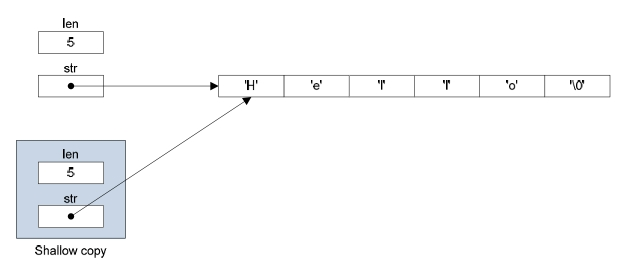
\includegraphics[width=1\textwidth]{pics/shallow_copy.jpg}
			\end{minipage}
			\hspace*{0.5cm}
			\begin{minipage}[t]{9cm}
				\vspace*{-0.3cm}\paragraph{Deep-Copy}
					\vspace*{-0.3cm}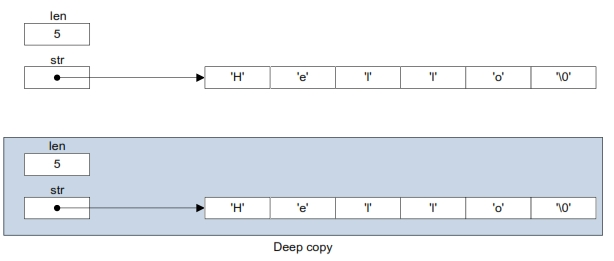
\includegraphics[width=1\textwidth]{pics/deep_copy.jpg}
			\end{minipage}
			
	\vspace*{-0.1cm}\subsection{Destruktor}
		\begin{compactitem}
			\item Vollst�ndige und "saubere" Zerst�rung eines nicht mehr ben�tigten Objekts
			\item Sie werden automatisch aufgerufen, wenn der G�ltigkeitsbereich des definierten Objekts ausl�uft
			\item Die h�uftigste Aufgabe ist die Freigabe von nicht mehr ben�tigten Speicher auf dem Heap
			\item sehr h�ufig (Wenn kein Speicher auf dem Heap vorhanden ist) wird kein Destruktor definiert, da das System dann automatisch aufr�umt
			\item Destruktoren haben keine Argumente und keine R�ckgabetypen
			\item Die Reihenfolge des Aufrufs der Destruktoren ist umgekehrt wie die der Konstruktoren. (das zuletzt erzeugte Objekt wird zuerst aufger�umt)
			\item sobald eine Methode mit $virtual$ gekennzeichnet ist, muss der Destruktor auch virtual sein.
		\end{compactitem}
		Folgend ein Beispiel, wie ein eigener D-tor im Headerfile implementiert wird:
		\lstinputlisting{code/destructor_bsp.cpp}
	
	\subsection{Member In-Class Initialization}
		\begin{minipage}[t]{9cm}
			\begin{compactitem}
				\item Ab $C++11$ k�nnen bei der Klassendeklaration den Attributen Initialisierungswerte zugewiesen werden.
				\item Implementationstechnisch sind sie �quivalent zur Initialisierungsliste bei C-tors
			\end{compactitem}
		\end{minipage}
		\hspace*{0.5cm}
		\begin{minipage}[t]{9cm}
			\vspace*{-0.8cm}\lstinputlisting{code/member_in_class_init.cpp}
		\end{minipage}
	
	\vspace*{-0.3cm}
	\subsection{kanonische Form von Klassen}
		\begin{compactitem}
			\item Die kanonische Form ist die Form, die es erlaubt, eine Klasse wie einen �normalen� Datentyp zu benutzen (ist f�r alle Klassen anzustreben).
			\item 3 Bedingungen:
			\begin{compactenum}
				\item Ein korrekter Default-Konstruktor, plus evtl. weitere Konstruktoren
				\item Bei dynamischen Daten, braucht es einen Zuweisungsoperator (sp�ter) und einen Copy-Konstruktor
				\item Ein (virtueller) Destruktor garantiert die korrekte Zerst�rung von Objekten
			\end{compactenum} 
		\end{compactitem}
		
	\subsection{Unions}
		\begin{compactitem}
			\item �hnlich wie Struktur
			\item im Gegensatz zur Struktur ist aber nur ein einziges Feld jeweils aktiv (abh�ngig vom Typ)
			\item Die Gr�sse einer Union ist so gross wie das gr�sste Feld der Union
			\item {\bf Vorsicht}, der Programmierer muss verfolgen, welcher Typ jeweils in der Union gespeichert ist. Der Datentyp, der entnommen wird, muss der sein, der zuletzt gespeichert wurde. 
		\end{compactitem}
		\begin{minipage}[t]{5 cm}
			\subsubsection{Beispiel}
				\vspace*{-0.3cm}
				\lstinputlisting{code/unions2.c}
		\end{minipage}
		\hspace*{0.5cm}	
		\begin{minipage}[t]{4.5 cm}
			\vspace*{0.1cm}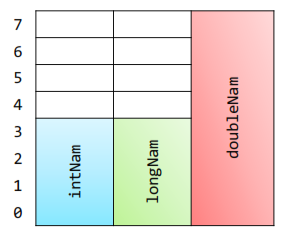
\includegraphics[width=\textwidth]{pics/union.png}
		\end{minipage}

	\subsection{Bitfelder}
		\begin{compactitem}
			\item Innerhalb eines int?s k�nnen einzelne Bitgruppen definiert und angesprochen werden
			\item Kann n�tzlich sein, wenn auf einzelne Bitgruppen in einem Register zugegriffen werden soll
			\item {\bf Achtung:} ist nicht definiert, ob die Bits von links oder von rechts aufgef�llt werden (Compilerabh�ngig)
			\item Sollte also nicht eingesetzt werden, wenn der Code portabel sein soll
			\item Der Datentyp eines Bits ist immer derselbe, wie das ganze Bitfeld gross ist
		\end{compactitem}
		\lstinputlisting{code/bitfeld.cpp}
	
	\subsection{�berladen von Operatoren}
		Operatoren (z.B. +, ==, etc.) k�nnen wie Funktionen �berladen werden.
		
		\subsubsection{�berladbare Operatorfunktionen in C++}
		\begin{minipage}[t]{3 cm}
			\begin{compactitem}
				\item \lc{new}
				\item \lc{delete}				
				\item \lc{new[ ]}				
				\item \lc{delete[ ]} 	
				\item \lc{+}
				\item \lc{-}							
			\end{compactitem}
		\end{minipage}
		\begin{minipage}[t]{2.1 cm}
			\begin{compactitem}	
				\item \lc{*}
				\item \lc{/}			
				\item \lc{\%}
				\item \lc{\textasciicircum}
				\item \lc{\&}	
				\item \lc{|}		
			\end{compactitem}
		\end{minipage}
		\begin{minipage}[t]{2.1 cm}
			\begin{compactitem}	
				\item \lc{\textasciitilde}
				\item \lc{!}	
				\item \lc{=} 			 	
				\item \lc{<} 	
				\item \lc{>}	 		 	
			\end{compactitem}
		\end{minipage}
		\begin{minipage}[t]{2.1 cm}
			\begin{compactitem}	
				\item \lc{+=}			 	
				\item \lc{-=}			 	
				\item \lc{*=}		
				\item \lc{/=}	
				\item \lc{\%=}		 	
			\end{compactitem}
		\end{minipage}
		\begin{minipage}[t]{2.1 cm}
			\begin{compactitem} 
				\item \lc{\textasciicircum=}			 	
				\item \lc{\&=} 		 	
				\item \lc{|=}			 	
				\item \lc{<<}		
				\item \lc{>>}	 	
			\end{compactitem}
		\end{minipage}
		\begin{minipage}[t]{2.1 cm}
			\begin{compactitem}		 
				\item \lc{>>=} 			 	
				\item \lc{<<=}			 	
				\item \lc{==} 			 	
				\item \lc{!=}
				\item \lc{<=}	
			\end{compactitem}
		\end{minipage}
		\begin{minipage}[t]{2.1 cm}
			\begin{compactitem}		 	
				\item \lc{>=} 		 	
				\item \lc{\&\&} 			 	
				\item \lc{||} 			 	
				\item \lc{++} 		
				\item \lc{--}	 	
			\end{compactitem}
		\end{minipage}
		\begin{minipage}[t]{2.4 cm}
			\begin{compactitem}		 	
				\item \lc{,} 			 	
				\item \lc{->*}	
				\item \lc{->}		 	
				\item \lc{()}
				\item \lc{[ ]}
			\end{compactitem}
		\end{minipage}
		
		\subsubsection{Randbedingungen}
		\begin{compactitem}
			\item Die Anzahl der Operanden (Argumente) muss gleich sein wie beim urspr�nglichen Operator.
			\item Die Priorit�t des �berladenen Operators kann nicht �ndern.
			\item Neue Operatoren k�nnen nicht eingef�hrt werden.
			\item Default-Argumente sind bei Operatoren nicht m�glich.
		\end{compactitem}
	
		\subsubsection{Operator Overloading als Elementfunktion}
		Der neu definierte Operator wird als Elementfunktion implementiert. Damit ist
		der Zugriff auf \lc{private} und \lc{protected} Attribute der Klasse m�glich.
		\lstinputlisting{code/operator_overloading_element.cpp}
		{\bf Achtung:} Zwingend als Elementfunktion zu implementieren sind: \\
		Zuweisungsoperator \lc{=}, Indexaufruf \lc{[ ]}, Funktionsaufruf \lc{()} und Zeigeroperator \lc{->}
		
		\subsubsection{Operator Overloading als normale Funktion}
		Die Operatorfunktionen werden meist als normale Funktion implementiert. Dadurch besteht jedoch kein Zugriff mehr auf die \lc{private} und \lc{protected} Elemente der Klasse. Die Operatorfunktion muss deshalb als \lc{friend} deklariert werden.
		\lstinputlisting{code/operator_overloading_normal.cpp}
		
	
	\newpage
\section{Templates}
	\subsection{Motivation}
		Wesentliche Vorteile von Templates sind:
		\begin{compactitem}
			\item {\bf Single-Source-Prinzip:} F�r x Varianten derselben Datenstruktur existiert genau eine Version des Sourcecodes, der ge�ndert und gewartet werden muss.
			\item {\bf H�here Wiederverwendbarkeit:} Klassen-Templates sind bei geeigneter Wahl ihrer Parameter allgemein einsetzbar und einfach wiederverwendbar.
			\item {\bf Statische Bindung:} Die Bindung zur �bersetzungszeit hat in Bezug auf Typsicherheit und Fehlererkennung zweifellos grosse Vorteile gegen�ber generischen C-L�sungen mit \lc{void*}-Zeigern, aber zum Teil auch gegen�ber typisch objektorientierten Varianten wie sie zum Beispiel in Smalltalk �blich sind.
			\item {\bf  Dead Code:} Traditionelle Bibliotheken belegen Speicher unabh�ngig davon, ob eine
			einzelne Funktion wirklich verwendet wird. Dies kann zu Dead Code f�hren,
			d.h. zu Code, der niemals ausgef�hrt wird.
		\end{compactitem}
		
	\subsection{Funktions-Templates}
		\begin{compactitem}
			\item Templates verwenden den Typ als Variable.
			\item Die Algorithmen k�nnen unabh�ngig vom Typ (generisch) implementiert
			werden.
			\item Templates sind keine Funktionsdefinitionen, sie beschreiben dem Compiler
			nur, wie er den Code definieren soll, d.h. der Compiler nimmt den konkret
			verwendeten Typ, setzt diesen in das Template ein und compiliert den so
			erhaltenen Code.
			\item Die Bindung zum konkreten Typ geschieht bereits zur Compiletime (early
			binding), sobald bekannt ist, mit welchem Typ das Template aufgerufen
			(benutzt) wird.
		\end{compactitem}
		
		\subsubsection{Syntax}
			\begin{minipage}[t]{10.5cm}
				\begin{compactitem}
					\item Vor den Funktionsnamen wird das Schl�sselwort \lc{template}, gefolgt von einer
					in spitzen Klammern eingeschlossenen Parameterliste gestellt.
					\item Die Parameterliste enth�lt eine (nicht leere) Liste von Typ- und
					Klassenparametern, die mit dem Schl�sselwort \lc{class} oder \lc{typename}
					beginnen. Die einzelnen Parameter werden mit Komma getrennt.
				\end{compactitem}
			\end{minipage}
			\hspace*{0.5cm}
			\begin{minipage}[t]{7cm}
				\vspace*{-0.5cm}\lstinputlisting[language=C++,tabsize=2]{code/template_syntax.cpp}
			\end{minipage} \\
			
		\vspace*{-0.1cm}\subsubsection{inline bei Templates}
			\lc{inline} muss zwischen \lc{template} und dem Returntyp stehen.
			Achtung: Bei Verwendung von \lc{inline} speziell zusammen mit Templates besteht die Gefahr von Code Bloat.

		\subsubsection{�berladen}
			\begin{compactitem}
				\item Funktions-Templates k�nnen mit anderen Funktionstemplates und auch mit normalen Funktionen �berladen werden.
				\item Namensaufl�sung:
				\begin{compactitem}
					\item Compiler geht Liste der m�glicherweise passenden Funktions-Templates durch und erzeugt die entsprechenden Template-Funktionen.
					\item Ergebnis ist eine Reihe von (eventuell) passenden Template-Funktionen, erg�nzt durch die vorhandenen normalen Funktionen.
					\item Aus dieser ganzen Auswahl wird die am besten passende Funktion ausgew�hlt.
				\end{compactitem}	
			\end{compactitem}
		
		\vspace*{-0.1cm}\begin{minipage}[t]{9cm}							
			\subsubsection{Auspr�gung}
				\begin{compactitem}
					\item Sobald ein Typ in einem Funktions-Template verwendet wird, erkennt der
					Compiler, dass es sich um ein Template handelt und pr�gt es f�r diesen Typ aus
					(implizite Auspr�gung).
					\item F�r die Aufl�sung werden nur die Funktionsparameter betrachtet, der
					R�ckgabetyp wird nicht ausgewertet.			
				\end{compactitem}
				\lstinputlisting[language=C++,tabsize=2]{code/template_auspraegung.cpp}
		\end{minipage}
		\hspace*{0.5cm}
		\begin{minipage}[t]{9cm}			
			\subsubsection{Explizite Qualifizierung}
				\begin{compactitem}
					\item Funktions-Templates k�nnen explizit mit einem Typ qualifiziert werden.		
				\end{compactitem}
				\lstinputlisting[language=C++,tabsize=2]{code/template_explizit.cpp}
		\end{minipage}
		
	\subsection{Klassen-Templates}
		\begin{minipage}[t]{7 cm}
			\subsubsection{Definition}
				\begin{compactitem}
					\item Klassen-Templates sind mit Typen oder Konstanten parametrisierbare Klassen.
					\item Im Gegensatz zu Funktions-Templates k�nnen in Klassen-Templates auch die
					Attribute der Klassen mit variablen Typen ausgestattet sein.
					\item Ein Klassen-Template kann auch von Ausdr�cken abh�ngig sein. Diese Ausdr�cke m�ssen aber zur Compiletime aufgel�st werden k�nnen.
				\end{compactitem}
				
			\subsubsection{Syntax}
				\begin{compactitem}
					\item Die Syntax ist analog zu den Funktions-Templates.
					\item Vor die Klassendeklaration wird das Schl�sselwort $template$, gefolgt von
					einer in spitzen Klammern eingeschlossenen Parameterliste gestellt.
					\item Die Parameterliste enth�lt eine (nicht leere) Liste von Typ- und
					Klassenparametern, die mit dem Schl�sselwort $class$ oder $typename$
					beginnen oder auch von Ausdr�cken. Die einzelnen Parameter werden mit Komma getrennt.
				\end{compactitem}
		\end{minipage}
		\hspace*{0.5cm}
		\begin{minipage}[t]{11 cm}
			\lstinputlisting[language=C++,tabsize=2]{code/template_class.cpp}
		\end{minipage}
		
	\vspace*{-0.2cm}\subsection{Klassen-Templates und getrennte �bersetzung}
		\vspace*{-0.4cm}\begin{minipage}[t]{9 cm}
			\subsubsection{M�glichkeit 1}
				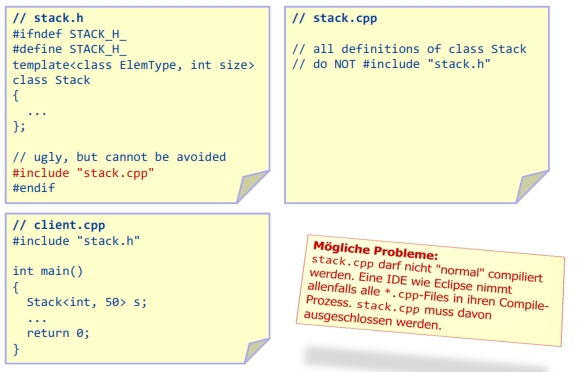
\includegraphics[width=\textwidth]{pics/template_klasse_1.jpg}
		\end{minipage}
		\hspace*{0.5cm}
		\begin{minipage}[t]{9 cm}
			\subsubsection{M�glichkeit 2}
				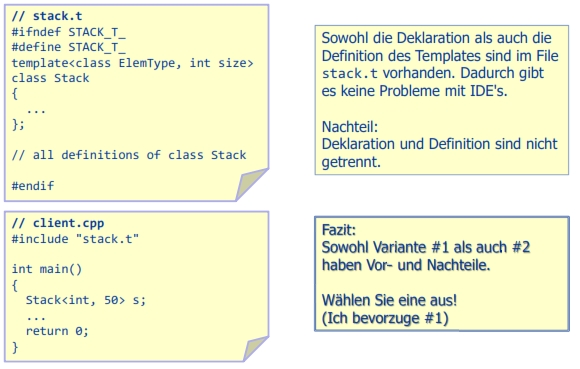
\includegraphics[width=\textwidth]{pics/template_klasse_2.jpg}
		\end{minipage}	
	
	\newpage
\section{Vererbung (Inheritance)}
	Vererbung ist ein Konzept, das es erlaubt, neue Klassen auf Basis von alten Klassen zu definieren. Die neuen (Unter-, Sub-) Klassen besitzen, ohne Eingriffe in den
	Sourcecode der bereits bestehenden (Ober-, Basis-, Super-) Klassen, all deren Eigenschaften, sie erben deren Verhalten und Daten. Den Vorgang der Vererbung nennt man auch Ableiten.\\
	\begin{minipage}[t]{7 cm}
		\subsection{Einsatz der Vererbung}
		\begin{compactitem}
			\item Bestehende Klassen erweitern (zus�tzliche Attribute und Elementfunktionen)
			\item Bestehende Methoden einer Basisklasse �ndern (�berschreiben)
			\item Einsatz nur wenn eine \textbf{IST-EIN} Beziehung besteht (z.B. Baum \textbf{ist eine} Pflanze, Blume \textbf{ist eine} Pflanze)\\
		\end{compactitem}
		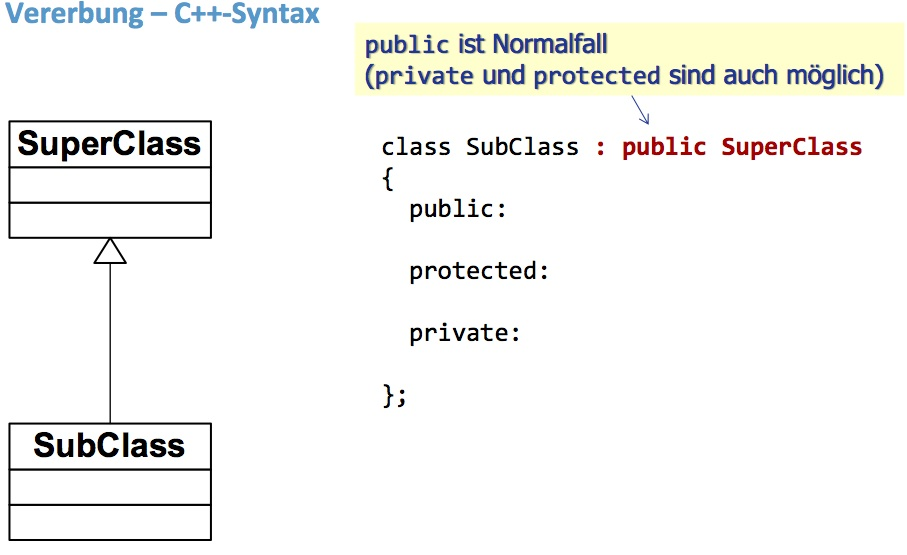
\includegraphics[width=1\textwidth]{pics/bsp_Vererbung.jpg}
		\subsection{Ableiten einer Klasse}
			Der Syntax der Ableitung einer Klasse ist oben aufgef�hrt. Als weiteres Beispiel ist im Anhang das Beispiel des \lc{ComicCharacters} und \lc{SuperHero} eingef�gt. \lc{SuperHero} \textbf{ist ein} \lc{ComicCharacter}.
			\begin{compactitem}
				\item \lc{friend}-Beziehungen werden nicht vererbt
				\item Ein Objekt einer Oberklasse kann Objekte einer beliebigen Unterklasse aufnehmen aber nicht umgekehrt (Substitutionsprinzip)
				\item Ein Objekt einer vererbten Klasse enth�lt alle Teile der Basisklasse und zus�tzlich noch die spezifischen eigenen Teile.
				\item Das Objekt ist somit mindestens so gross wie jenes der Basisklasse (es gibt keine Vererbung \lc{by reference})
				\linebreak
			\end{compactitem}
			\lstinputlisting[language=C++,tabsize=2]{code/substitutionsprinzip.cpp}
	\end{minipage}	
	\hspace*{0.5cm}
	\begin{minipage}[t]{11.5 cm}
	\subsection{Zugriff auf Elemente der Basisklasse}
		\textbf{Bei Vererbung mit \lc{public} (Normalfall):}
			\begin{compactitem}
				\item Zugriff m�glich auf alle \lc{public}- und \lc{protected}- Elemente der Basisklasse, die Zugriffsrechte 
				(\lc{public}, \lc{protected}) der Basisklasse werden in der abgeleiteten Klasse beibehalten
				\linebreak
			\end{compactitem}
		\textbf{Bei Vererbung mit \lc{protected}:}
			\begin{compactitem}
				\item Zugriff m�glich auf alle \lc{public}- und \lc{protected}- Elemente der Basisklasse, die Zugriffsrechte 
				von \lc{public} und \lc{protected} der Basisklasse werden in der abgeleiteten Klasse zu \lc{protected}
				\linebreak
			\end{compactitem}
		\textbf{Bei Vererbung mit \lc{private}:}
			\begin{compactitem}
				\item Zugriff m�glich auf alle \lc{public}- und \lc{protected}- Elemente der Basisklasse, die Zugriffsrechte von \lc{public} und \lc{protected} der Basisklasse werden in der abgeleiteten Klasse zu \lc{private}
				\linebreak
			\end{compactitem}
		\textbf{Bei allen drei: kein Zugriff auf \lc{private}-Elemente der Basisklasse}
		%\lstinputlisting[language=C++,tabsize=2]{code/privateFehler.cpp}
		\vspace*{0.3cm}
		\subsection{Slicing Problem}
			Links: Beim Kopieren werden nur die \lc{ComicCharacter}-Teile ber�cksichtigt. Durch das Kopieren wird alles �berfl�ssige 
			weggeschnitten, �brig bleibt ein reines \lc{ComicCharacter} Objekt im Fall von \lc{s} f�hrt dies dazu, dass die erweiterten \lc{SuperHero} Daten und Funktionen verloren gehen.\newline
			Rechts: Hier wird dank des Referenzparameters der gesamte Superheld ausgegeben.\newline
			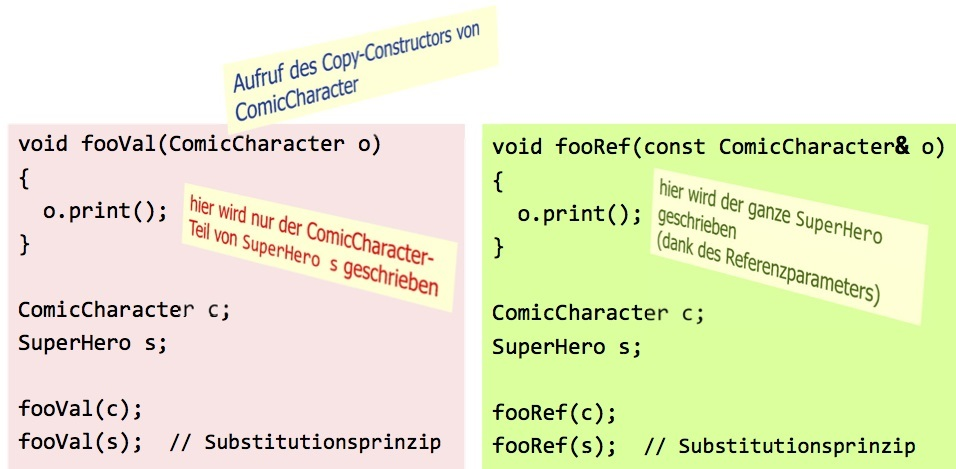
\includegraphics[width=1\textwidth]{pics/SlicingProblem.jpg}
		%\end{minipage}	
		\subsection{Vererbung und G�ltigkeitsbereiche}
			Die Klasse \lc{C} enth�lt alle Elemente von \lc{B} und somit auch von \lc{A}. \lc{A} jedoch hat kein \lc{i} und kann auch von keiner Oberklasse erben, dies ergibt den Fehler. \lc{B} hat zwar auch kein \lc{j}, erbt aber das von \lc{A}.\newline
			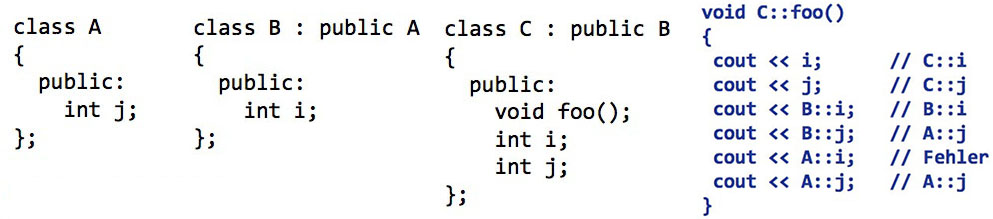
\includegraphics[width=1\textwidth]{pics/zugriffVererbung.jpg}
	\end{minipage}
	\subsection{Elementfunktionen bei abgeleiteten Klassen}
	\vspace*{-0.4cm}
	\begin{minipage}[t]{12 cm}
    	\subsubsection{Konstruktoren}
    		In einem Konstruktor m�ssen alle Elemente eines Objekts (auch die ererbten) initialisiert werden. Folgendes Beispiel zeigt die direkte Initialisierung aller Elemente. Vor allem bei grossen oder mehreren Klassen ist dies nicht zielf�hrend. Stattdessen wird das Chaining Prinzip angewandt. Falls kein Aufruf eines Basislklassen-Konstruktors in der Initialisierungsliste eines Konstruktors erscheint, so f�gt der Compiler automatisch den Default-Konstruktor der Basisklasse ein.
   			\lstinputlisting[language=C++,tabsize=2]{code/initVererbungKonstruktor.cpp}
   		\subsubsection{Initialisierung durch Chaining}
   			Jede Klasse erledigt nur die eigenen Aufgaben. Aufgaben, die ererbte Methoden �bernehmen k�nnen, werden diesen delegiert (Aufruf der jeweiligen Konstruktoren)\newline
   			\textbf{Wichtig: die Elemente der Basisklasse m�ssen immer als erste initialisiert werden}
    		\lstinputlisting[language=C++,tabsize=2]{code/initVererbungChaining.cpp}
	\end{minipage} \hspace*{0.5cm}
	\begin{minipage}[t]{6.5 cm}
		\subsubsection{Copy-Konstruktor}
			\begin{compactitem}
				\item Wenn kein Copy Constructor explizit definiert wird, so erzeugt das System einen
				\item Darin wird immer (ebenfalls automatisch) zuerst der Copy Constructor der Basisklasse aufgerufen
				\linebreak
			\end{compactitem}
		\subsubsection{Destruktor}
			\begin{compactitem}
				\item Auch Destruktoren werden nach dem Chaining-Prinzip aufgebaut
				\item Jede Klasse k�mmert sich um die eigenen Attribute und �berl�sst jene der
				Basisklasse auch der Basisklasse
				\item Destruktoren m�ssen nie explizit aufgerufen werden. Der Destruktor der
				Basisklasse wird \textbf{am Schluss} des Destruktors immer automatisch aufgerufen\newline
				Ein leerer Destruktor der Art
				\lstinputlisting[language=C++,tabsize=2]{code/destructor.cpp}
				ruft automatisch den Basisklassen-Destrukor (von \lc{ComicCharacter}) auf.
				\\
			\end{compactitem}
		\subsubsection{�berschreiben von ererbten Methoden}
			\begin{compactitem}
				\item Falls ererbte Methoden nicht das erf�llen, was eine bestimmte Klasse m�chte, dann
				k�nnen diese Methoden neu definiert (�berschrieben) werden.
				\item Methoden, welche in einer abgeleiteten Klasse �berschrieben werden k�nnen, m�ssen in der Basisklasse mit \lc{virtual} gekennzeichnet sein.
				\item Ab \lc{C++11} sollen in der Unterklasse die �berschriebenen Methoden mit \lc{override} gekennzeichnet werden. Damit weiss der Compiler, dass mit dieser Methode eine andere �berschrieben wird.
				\item Im Anhang wird dieses �berschreiben einer Methode beim \lc{SuperHero} f�r die Funktion \lc{dance()} vorgenommen. W�hrend ein normaler \lc{ComicCharacter} tanzt, wird diese Funktion beim \lc{SuperHero} �berschrieben und mit tanzt nicht �berschrieben.
				\linebreak
			\end{compactitem}		
	\end{minipage}   
	
	\newpage
\section{Polymorphismus / Mehrfachvererbung / RTTI}
   		Dieses Kapitel beschreibt die dynamischen objektorientierten Sprachmerkmale von \lc{C++}. Erst durch diese wird \lc{C++} zu einer echten objektorientierten Programmiersprache.\\
	%\begin{minipage}[t]{8 cm}
	\subsection{Polymorphismus}
		\begin{minipage}[t]{9cm}
			\subsubsection{Problem}
			\begin{compactitem}
				\item Abstrakter Auftrag, aber die Ausf�hrung ist bereits sehr konkret.
				\item Eine immer gleich heissende Elementfunktion hat unterschiedliche Implementationen, je nach Art des aktuellen Objekts.
			\end{compactitem}
			\subsubsection{static Binding}
			Ist der Normalfall und wird auch early Binding genannt. Hier wird bereits zur Compilezeit festgelegt, welcher Code ausgef�hrt wird.
			\subsubsection{dynamic Binding}
			\begin{compactitem}
				\item Erst zu Laufzeit wird in Abh�ngigkeit des Objekts festgelgt, welcher Code ausgef�hrt wird.
				\item Das ist das Konzept des Polymorphismus.
				\item Der m�chtigste OO-Mechanismus (oft pr�ziser mit run-time polymorphism bezeichnet)
				\item Regeln:
				\begin{compactitem}
					\item Eine Funktion soll dann virtual deklariert werden, wenn sie in der abgeileiteten Klasse neu	definiert (�berschieben) wird, sonst nicht!
					\item Wenn mindestens eine Elementfunktion virtual ist, muss auch der Destruktor virtual sein.
					\item Der Destruktor muss auch dann virtual sein, wenn ein Objekt einer Unterklasse dynamisch erzeugt wird und einem Pointer auf die Basisklasse zugewiesen wird (Substitutionsprinzip)
					\\
				\end{compactitem}
			\end{compactitem}
		\end{minipage}
		\hspace*{0.5cm}
		\begin{minipage}[t]{9	cm}
			\subsubsection{Beispiel}
				\begin{compactitem}
					\item Der statische Datentyp bezeichnet den Datentyp bei der Deklaration. Im Beispiel: \lc{a} ist ein Array von Pointer auf \lc{Article}
					\item Der dynamische Datentyp bezeichnet den effektiven Datentyp zur Laufzeit Im Beispiel: \lc{a[0]} ist ein Pointer auf \lc{Book}, \lc{a[1]} ein Pointer auf \lc{CD}, etc.
				\end{compactitem}
				\includegraphics[width=1\textwidth]{pics/bsp_Webshop.jpg}
		\end{minipage}
		
	\begin{minipage}[t]{7 cm}
		\subsubsection{Polymorphe (virtuelle) Klassen}
			\begin{compactitem}
		 		\item Eine Klasse, welche mindestens eine virtuelle Funktion deklariert, heisst virtuell (polymorph)
				\item Virtuelle Klassen bewirken einen Mehraufwand f�r den Compiler und sind darum langsamer in der Ausf�hrung
				\item Konstruktoren sind nie virtuell
				\item Destruktoren virtueller Klassen m�ssen immer als virtuell deklariert werden,
				sonst wird nur der Destruktor der Basisklasse aufgerufen
				\item \textbf{Nicht virtuelle Methoden d�rfen nicht �berschrieben werden} (k�nnten technisch gesehen, f�hrt aber zu un�berschaubaren Fehlern)
				\item In der Unterklasse sollen die �berschriebenen Methoden mit override gekennzeichnet werden. Dient der �bersicht und wenn die zu �berschreibenden Methode in der Basisklasse nicht virtuell ist, ruft der
				Compiler aus.
			\end{compactitem}
	\end{minipage}
	\hspace*{0.5cm}
	\begin{minipage}[t]{11 cm}
		\subsubsection{Repr�sentation polymorpher Objekte im Speicher}
			\begin{compactitem}
				\item In der Virtual Function Table (vtbl) vermerkt das System der Reihe nach die Adressen der f�r eine Klasse g�ltigen virtuellen Elementfunktionen
				\item Das System legt f�r jede polymorphe Klasse eine vtbl an
				\item Jedes Objekt einer polymorphen Klasse enth�lt einen Virtual Pointer vptr, welcher auf die vtbl der entsprechenden Klasse zeigt
			\end{compactitem}
		\hspace*{0.5cm}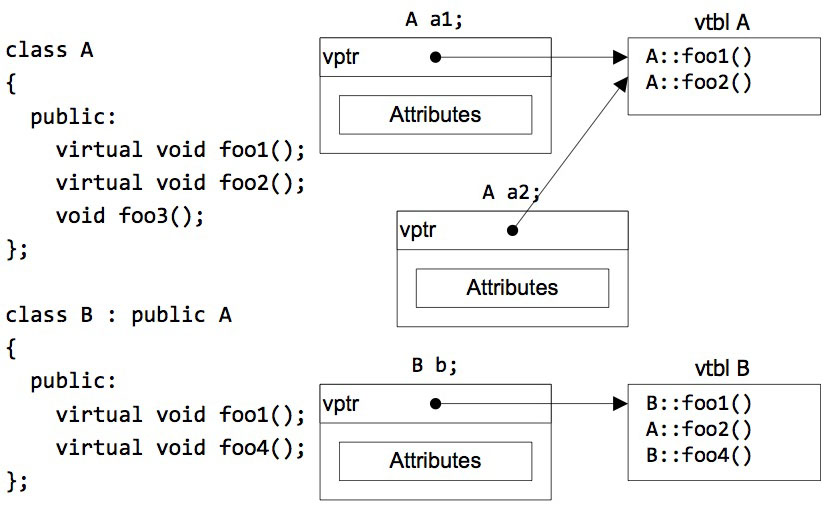
\includegraphics[width=1\textwidth]{pics/bsp_vtbl.jpg}
	\end{minipage}
	\subsection{Abstrakte Klassen}
		Eine abstrakte Klasse ist ein Klasse, die mehr oder weniger vollst�ndig ist und dazu dient, Gemeinsamkeiten der abgeleiteten Klassen festzuhalten (z.B. \lc{ComicCharacter}). \lc{ComicCharacter} legt fest, dass alle Comicfiguren die Methoden \lc{print()}, \lc{dance()} und \lc{sing()} verstehen.
		\begin{compactitem}
			\item Ein Kreis ist z.B. ein Spezialfall einer Ellipse. Es ist aber nicht sinnvoll, ihn so zu programmieren, da er sonst Eigenschaften erbt, die nicht verwendet werden
			\item Es w�re m�glich, Kreis und Ellipse als zwei unabh�ngige Klassen zu programmieren. Dann m�ssten aber alle Eigenschaften, die diese gemeinsam haben, doppelt programmiert werden
			\item Dies versucht die objektorientierte Programmierung zu vermeiden
			\item Es ist besser, die Eigenschaften, die Kreise und Ellipsen gemein haben, in einer Basisklasse zu programmieren
			\item Die Kreis- und Ellipsenklasse erben dann parallel von der gemeinsamen Basisklasse
			\item Die Basisklasse ist aber unvollst�ndig, es handelt sich um eine abstrakte Klasse
			\item Es k�nnen \textbf{keine} Objekte von abstrakten Klassen gebildet werden
			\item In \lc{C++} k�nnen rein virtuelle Funktionen (pure virtual functions) deklariert werden, die in der Basisklasse nicht von einer Definition begleitet werden. Beispiel:
			\lstinputlisting[language=C++,tabsize=2]{code/pure_virtual_function.cpp}
			\textbf{\item Klassen, die mindestens eine rein virtuelle Funktion deklarieren, sind abstrakte Klassen}
			\item Ist eine Klasse erst einmal als abstrakt definiert, kann diese nur durch Vererbung vervollst�ndigt und dadurch nutzbar gemacht werden \\
		\end{compactitem}
		
	\subsection{Mehrfachvererbung}
		\begin{minipage}[t]{6.5 cm}
		Bei der Mehrfachvererbung wird eine Klasse von mehreren Basisklassen abgeleitet. So kann z.B. eine Klasse \lc{DuckHero} definiert werden, die sowohl von \lc{SuperHero} als auch von \lc{SingingComicCharacter} erbt. \\
		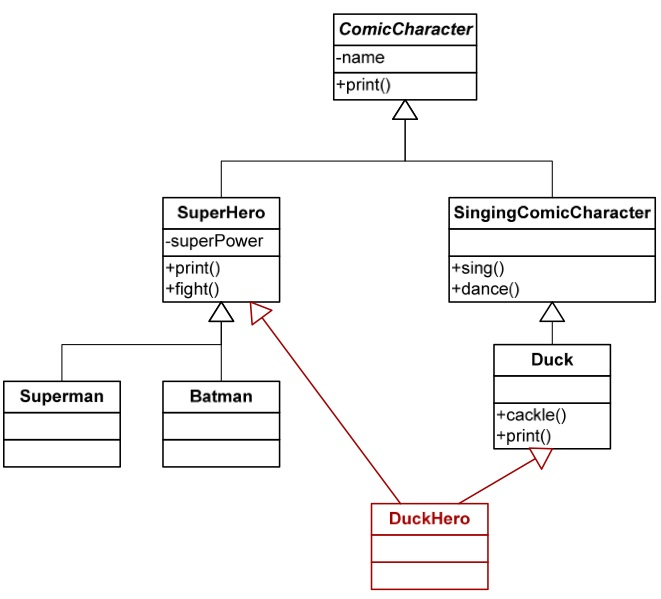
\includegraphics[width=1\textwidth]{pics/uml_mehrfachvererbung.jpg}
		Guter Einsatz der Mehrfachvererbung ist, wenn alle ausser h�chstens einer Basisklasse ausschliesslich aus rein virtuellen Funktionen bestehen (Interfaces). Die neue Klasse implementiert dann die aufgelisteten Interfaces.\\
		Das obige Beispiel ist im Anhang unter 15.4 angeh�ngt.
		\end{minipage}\hspace*{0.5cm}
		\begin{minipage}[t]{11.5 cm}
			Der Syntax bei der Mehrfachvererbung lautet wie folgt (Basisklassen durch Komma getrennt). Dabei m�ssen die Konstruktoren der Basisklassen in der Ordnung gelistet werden, in der sie aufgerufen werden sollen:
			\lstinputlisting[language=C++,tabsize=2]{code/mehrfachvererbung.cpp}
			Durch die Mehrfachverbung treten oft Probleme auf. Problem 1 ist jenes der Mehrdeutigkeit von Methoden. Im Fall von \lc{print()} ergeben sich mehrere M�glichkeiten. Um die Mehrdeutigkeit zu umgehen, muss der G�ltigkeitsbereich angegeben werden:
			\lstinputlisting[language=C++,tabsize=2]{code/mehrdeutigkeit.cpp}
			Oder noch besser:
			\lstinputlisting[language=C++,tabsize=2]{code/mehrdeutigkeit2.cpp}
			Das Problem 2 ist das von mehrfachen Basisklassen (linker und rechter Baum). \lc{DuckHero} ist von \lc{Duck} und \lc{SuperHero} abgeleitet und beinhaltet somit zwei \lc{ComicCharacter}-Teile. Diese Mehrdeutigkeit kann durch virtuelles erben verhindert werden. Dies muss jedoch bereits eine Stufe h�her geschehen.
		\end{minipage}
\newpage
	\subsection{RTTI (Laufzeit-Typinformation)}
	RTTI (Run-Time Type Information) ist die M�glichkeit den Typ eines Objekts einer polymorphen Klasse festzustellen. Er steht ausschliesslich f�r polymorphe Klassen zur Verf�gung und sollte sehr zur�ckhaltend eingesetzt werden.\linebreak
	Der RTTI-Mechanismus besteht im Wesentlichen aus zwei Operatoren und einer Struktur:
		\begin{compactitem}
			\item Operator \lc{dynamic\_cast}
			\item Operator \lc{typeid}
			\item Klasse \lc{type\_info}
		\end{compactitem}
	\subsubsection{Operator dynamic\_cast}
	Syntax: 	\lstinputlisting[language=C++,tabsize=2]{code/dynamic_cast.cpp}
		\begin{compactitem}
			\item Versucht, den Zeiger \lc{p} in einen Zeiger auf ein Objekt des Typs \lc{SuperHero}
			umzuwandeln
			\item Der dynamische Datentyp von \lc{p} ist massgebend
			\item Umwandlung wird dann durchgef�hrt, wenn \lc{p} tats�chlich auf ein Objekt vom Typ \lc{SuperHero}, bzw. auf eine davon abgeleitete Klasse zeigt.
			\item Andernfalls ist das Resultat der Umwandlung der Nullpointer!
		\end{compactitem}
	\subsubsection{Operator typeid}
		\begin{compactitem}
			\item Ermitteln des dynamischen Datentyps eines polymorphen Objekts
			\item Ergibt eine Referenz auf ein Objekt des Typs \lc{type\_info}. Diese Klasse beinhaltet u.a. eine Methode \lc{name()}, welche den Namen der Klasse zur�ckgibt.
		Beispiel: \lstinputlisting[language=C++,tabsize=2]{code/typeid.cpp}
		\end{compactitem}
	\subsubsection{Struktur type\_info}
		Die Struktur muss eingebunden werden
		\lstinputlisting[language=C++,tabsize=2]{code/type_info.cpp}
		Sie bietet mind. folgende Funktionalit�t:
		\begin{compactitem}
			\item die Operatoren \lc{==} und \lc{!=}
			\item die Methode \lc{before}
			\item die Methode \lc{name} (siehe Beispiel oben)
		\end{compactitem}
	
\vspace*{1.5cm}\section{Assertions}
	Um Assertions �berhaupft nutzen zu k�nnen muss zuerst die entsprechende Bibliothek eingebunden werden:
	\lstinputlisting{code/assert_include.cpp}
	Assertions dienen zur �berpr�fung von logischen Annahmen w�hrend der Entwicklungsphase, speziell f�r die �berpr�fung von Anfangs- und Endbedingungen in einer Funktion. Wenn die Bedingung \lc{false} ist, bricht das Programm ab. Es darf aber kein Nebeneffekt hineinprogrammiert werden, da asserts in der Release-Funktion wirkungslos sind.\\
	Beispiel:
	\lstinputlisting{code/assert.cpp}
	\subsection{\lc{static\_assert}}
		Diese Art von Assertions werden bereits zur Compilezeit �berpr�ft und man kann eine Textmeldung ausgeben falls Bedingung \lc{false} ist. Da die Bedingung zwingend zur Compilezeit auswertbar sein muss, darf sie keine Variablen o.�. beinhalten. Werden vorallem im Zusammenhang mit Templates genutzt.\\
		Beispiel:
		\lstinputlisting{code/assert_static.cpp}
	
	\newpage
\section{Exception Handling}
	Abnormale aber vorhersebare und m�gliche Bedingung bei der Programmausf�hrung.\\
	\begin{minipage}[t]{11cm}
		\subsection{Handling Strategie von System Exceptions}
			\begin{compactitem}
				\item In \lc{Java} und \lc{C\#} gelangen die System Exceptions in die Sprache, d.h. eine LowLevel Exception wird in eine Exception der Programmiersprache gemappt.
				\item Die Sprache \lc{C++} betreibt kein solches Exception Mapping, d.h. Low-Level 
				Exceptions werden nicht von \lc{C++} geworfen und k�nnen auch nicht mit
				\lc{catch(...)} abgefangen werden.
				\item Der Hauptgrund daf�r ist einmal mehr Effizienz. Wenn st�ndig Exceptions
				herumfliegen (auch wenn sie nicht abgefangen werden), dann beeintr�chtigt
				das die Performance.
				\item Einzelne Systemumgebungen betreiben dennoch Exception Mapping in \lc{C++}
				(z.B. \lc{Microsoft} in \lc{Visual C++}).
			\end{compactitem}
	\end{minipage}
	\hspace*{0.5cm}
	\begin{minipage}[t]{7cm}
		\subsection{Ziel}
		\begin{compactitem}
			\item Der Normalfall soll einfach gelesen werden k�nnen
			\item Der Ausnahmefall ist klar und einfach geregelt
			\item Der Overhead soll m�glichst klein sein
			\item Die Weiterreichung an die n�chsth�here Funktion im Call Stack soll einfach sein
		\end{compactitem}
	\end{minipage}

	\subsection{Exceptionhandling in \lc{C++}}
	\begin{compactitem}
		\item Exceptions werden in Form eines Objekts am Ort ihres Auftretens ausgeworfen (explizit oder auch "automatisch").
		\item Exception Handler versuchen, diese Exception-Objekte aufzufangen.
	\end{compactitem}

	\begin{minipage}[t]{9 cm}
		\subsubsection{Ausl�sen (Werfen) von Ausnahmen}
			\begin{compactitem}
				\item Ausnahmen k�nnen mit dem Schl�sselwort \lc{throw} explizit ausgeworfen werden.
				\item Nach einem \lc{throw}-Befehl wird das Programm abgebrochen und beim ersten passenden umgebenden Handler fortgesetzt.
				\item Dabei werden alle lokalen Objekte wieder automatisch zerst�rt (Stack unwinding).
				\item Geworfen werden kann ein beliebiges Objekt (�blich: ein spezifisches \lc{C++}-Ausnahmeobjekt).
				\item (Ausschliesslich) innerhalb eines Exception Handlers ist auch die Form
				\lc{throw;} erlaubt. Dadurch wird die Exception an den	n�chsten Handler weitergereicht (Exception propagation).
			\end{compactitem}	
	\end{minipage}
	\hspace*{0.5cm}
	\begin{minipage}[t]{9 cm}
		\subsubsection{Syntax}
			\lstinputlisting[language=C++,tabsize=2]{code/exception_handling.cpp}
	\end{minipage}
	\\
	
	\begin{minipage}[t]{11 cm}
		\subsubsection{Exception-Hierarchie in \lc{C++} und ihre Headers}		 	
			Ausnahmeobjekte k�nnen beliebigen Typs sein (z.B. auch \lc{int}). Meist werden jedoch spezifische hierarchisch organisierte Ausnahmeklassen verwendet.\\
			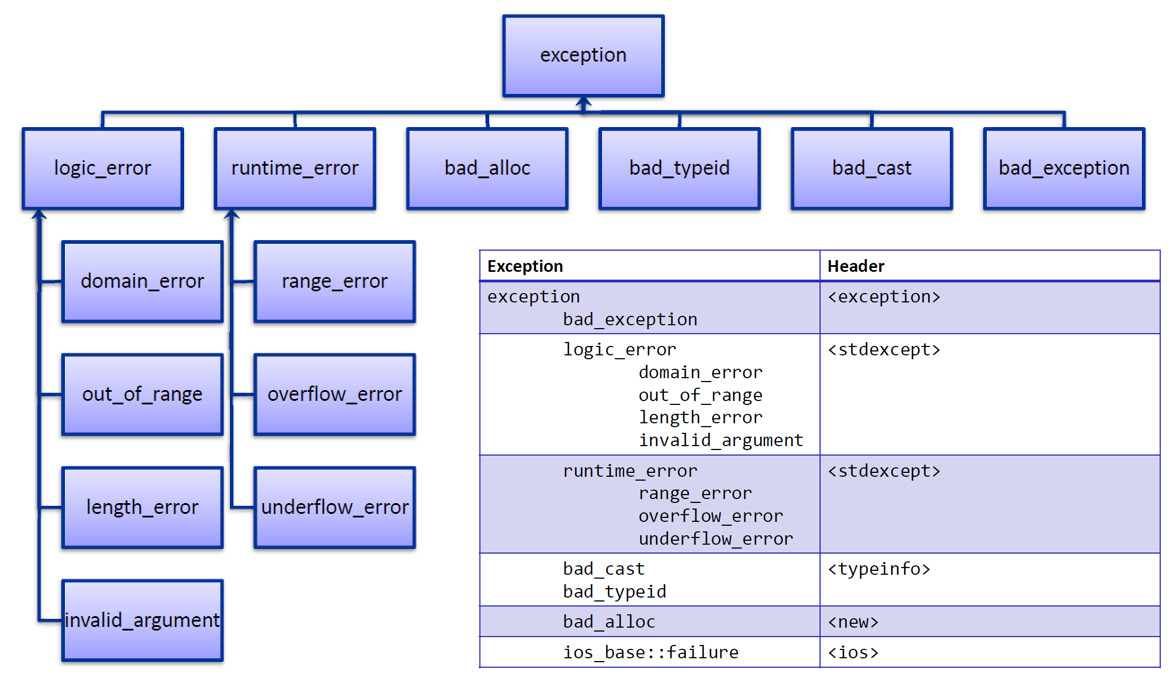
\includegraphics[width=1\textwidth]{pics/exception_hierarchy.png}
	\end{minipage}
	\hspace*{0.5cm}
	\begin{minipage}[t]{7 cm}
		\subsubsection{Laufzeit- vs. Logische Fehler}
			\begin{compactitem}
				\item Logische "Fehler" (logic\_error)
				\begin{compactitem}
					\item Ausnahmen im Programmablauf, die bereits zur Entwicklungszeit ihre Ursache	haben.
					\item Theoretisch k�nnten diese Ausnahmen verhindert werden.
				\end{compactitem}
				\item Laufzeit "Fehler" (runtime\_error)
				\begin{compactitem}
					\item Nicht vorhersehbare Ausnahmen wie z.B. arithmetische �berl�ufe.
					\item Diese Ausnahmen treten erst zur Laufzeit auf, z.B. durch eine nicht erlaubte Benutzereingabe.
				\end{compactitem}
			\end{compactitem}
	\end{minipage}
	
	%\begin{minipage}[t]{9 cm}
	\newpage
		\subsubsection{Mehrere Catches}
			\begin{compactitem}
				\item Ein oder mehrere Exception Handler k�nnen hintereinander definiert werden.
				\item Die einzelnen \lc{catch}-Handler m�ssen sich in den Parametern unterscheiden.
				\item Wenn eine Exception geflogen kommt, wird der erste passende Handler
				genommen. Ein passender Handler macht ein \lc{catch} auf genau diese Exception oder auf eine Basisklasse derselben.
				\item Deshalb (sehr wichtig): Der allgemeinste Handler (am meisten oben in der Hierarchie) muss als letzter definiert werden.
				\item Wenn kein Handler passt, dann wird im Aufrufstack nach oben gesucht, ob ein	passender Handler vorhanden ist.
				\item Wenn auch dort keiner gefunden wird, dann wird die Funktion \lc{terminate()} aufgerufen.
				\item \lc{terminate()} beendet das Programm, kann aber auch selbst definiert werden.
				\item Catch all: Der folgende Handler f�ngt ausnahmslos alle Exceptions ab (und muss wenn gew�nscht deshalb immer als letzter aufgef�hrt werden):	
			\end{compactitem}
			
			\hspace*{0.8cm}
			\begin{minipage}[t]{4cm}
				\lstinputlisting{code/catch_all.cpp}
			\end{minipage}
			\hspace*{3cm}
			\begin{minipage}[t]{10cm}
				\vspace*{-0.3cm}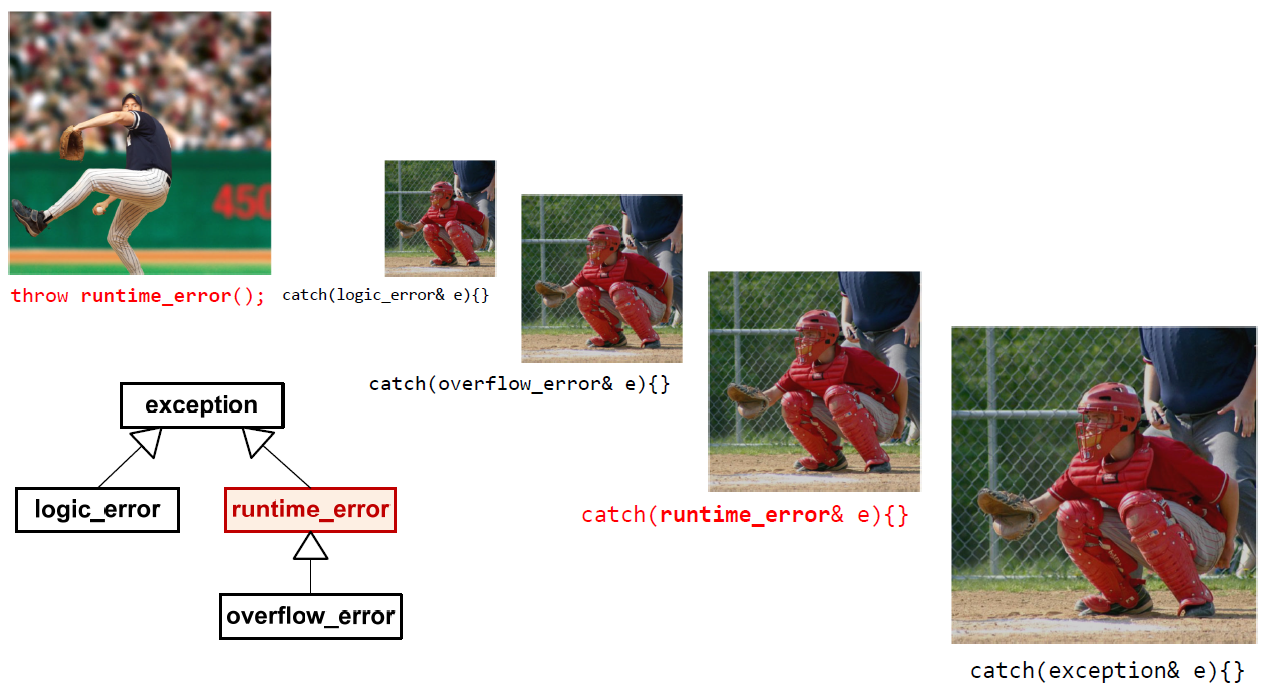
\includegraphics[width=\textwidth]{pics/exceptions.png}
			\end{minipage}
									
		\vspace*{-0.8cm}\paragraph{Exception Specification}
			\lc{void foo() throw(/* Liste der Exceptions */);}
			\begin{compactitem}
				\item Liste beschreibt, welche Exceptions von einem Aufrufer von \lc{foo()} erwartet werden m�ssen.
				\item Aber: garantiert auch, dass das Programm abst�rzt, wenn eine andere als die	spezifizierten Exceptions ausgeworfen wird, d.h. \lc{foo()} muss daf�r sorgen, dass wirklich nur die aufgelisteten Exceptions ausgeworfen werden.
				\item Genauer: falls eine nicht spezifizierte Exception ausgeworfen wird, dann wird die Funktion \lc{unexpected()} aufgerufen, welche �blicherweise das Programm abbricht.
				\item \lc{unexpected()} kann selbst definiert werden.
				\item {\bf Ab \lc{C++11} gilt jedoch:}
				\begin{compactitem}
					\item Exception Specifications sind deprecated (sollen nicht mehr verwendet werden)
					\item Aber: daf�r wurde ein neues Schl�sselwort \lc{noexcept} eingef�hrt, um anzugeben, dass eine Funktion keine
					Exceptions auswirft (na ja)
					\item \lc{noexcept} ist auch ein Operator, dem als Argument ein Funktionspointer �bergeben werden kann
					\begin{compactitem}
						\item returns \lc{true}, falls Funktion mit \lc{noexcept} spezifiziert ist
						\item sonst \lc{false}
					\end{compactitem}
				\end{compactitem}
			\end{compactitem}
	%\end{minipage}
	%\hspace*{0.5cm}
	%\begin{minipage}[t]{10 cm}
		\vspace*{0.2cm}
		{\bf Beispiele:}
		\lstinputlisting{code/exception_specification.cpp}
		{\bf Beispiele ab \lc{C++11}:}
		\lstinputlisting{code/exception_specification_11.cpp}
	%\end{minipage}
	
	\section{Beispiele}
	\subsection{Stack als Klasse}
		\lstinputlisting{code/example_stack_header.cpp}
		\newpage\lstinputlisting{code/example_stack_source.cpp}
	
\newpage	
	\subsection{Stack als Template}
		\lstinputlisting{code/example_stack_template_header.cpp}
		\newpage\lstinputlisting{code/example_stack_template_source.cpp}
		
\newpage
 	\subsection{Vererbung Comiccharacter}
 		\lstinputlisting{code/Vererbung/ComicCharacter.h}
 		\lstinputlisting{code/Vererbung/ComicCharacter.cpp}
 		\lstinputlisting{code/Vererbung/SuperHero.h}
 		\lstinputlisting{code/Vererbung/SuperHero.cpp}
 		\lstinputlisting{code/Vererbung/ComicTest.cpp}
 		
\newpage
	\subsection{Mehrfachvererbung Comiccharacter}
	 	\lstinputlisting{code/Polymorphismus/ComicCharacter.h}
	 	\lstinputlisting{code/Polymorphismus/ComicCharacter.cpp}
		\lstinputlisting{code/Polymorphismus/SuperHero.h}
 		\lstinputlisting{code/Polymorphismus/SuperHero.cpp}
 		\lstinputlisting{code/Polymorphismus/SingingComicCharacter.h}
 		\lstinputlisting{code/Polymorphismus/SingingComicCharacter.cpp}
 		\lstinputlisting{code/Polymorphismus/Duck.h}
 		\lstinputlisting{code/Polymorphismus/Duck.cpp}
 		\lstinputlisting{code/Polymorphismus/DuckHero.h}
 		\lstinputlisting{code/Polymorphismus/DuckHero.cpp}
 		\newpage\lstinputlisting{code/Polymorphismus/ComicTest.cpp}
 		
\newpage
	\subsection{RTTI}
	 	\lstinputlisting{code/DynCastTest.cpp}
				

\end{document}
